% !Mode:: "TeX:UTF-8"
\documentclass[10pt,a4paper,notitlepage]{report}
\usepackage{ifxetex,ifluatex}

\newif\ifxetexorluatex
\ifxetex
  \xetexorluatextrue
\else
  \ifluatex
    \xetexorluatextrue
  \else
    \xetexorluatexfalse
  \fi
\fi

% Better rendition of computer modern.
\usepackage{lmodern}

\ifxetexorluatex
    \usepackage{fontspec}
\else
    \usepackage[utf8]{inputenc}
\fi

% For mathematical typesetting.
\usepackage{amsfonts,amsmath,amsfonts,amssymb}

% For formal grammar.
\usepackage{syntax}

% For typeset diagrams
\usepackage{bytefield}
\usepackage{dirtree}

% Provides an extended tabular environment.
\usepackage{booktabs}
\usepackage{tabularx}
\usepackage{ltablex}

% For images.
\usepackage{graphicx}
\usepackage{float}

% Put bibliography in ToC
\usepackage[nottoc]{tocbibind}

% For better enumerations.
\usepackage{enumitem}

% For verbatim text.
\usepackage{fancyvrb}

% For source code listings.
\usepackage{listings}

% For fancy captions.
\usepackage{caption}

% For hyperlinks and fancy citations.
\usepackage[colorlinks=true,linkcolor=black,citecolor=blue,urlcolor=blue]{hyperref}

% Setting page geometry.
\usepackage[left=4cm,right=2cm,top=2cm,bottom=2cm]{geometry}

% Default caption form
\captionsetup{labelfont=bf,textfont=it,justification=centering,font=footnotesize}

% Shamelessly pinched from 'dbaupp'. cheers!
% http://tex.stackexchange.com/questions/51645/x86-64-assembler-language-dialect-for-the-listings-package
\lstdefinelanguage
    [x64]{Assembler}     % add a "x64" dialect of Assembler
    [x86masm]{Assembler} % based on the "x86masm" dialect
    {   % with these extra keywords:
        morekeywords={
            CDQE,CQO,CMPSQ,CMPXCHG16B,JRCXZ,LODSQ,MOVSXD,
            POPFQ,PUSHFQ,SCASQ,STOSQ,IRETQ,RDTSCP,SWAPGS,
            SYSCALL,
            rax,rdx,rcx,rbx,rsi,rdi,rsp,rbp,
            r8,r8d,r8w,r8b,r9,r9d,r9w,r9b
        }
    }

% Alias python [2] to python. Add missing yield
\lstdefinelanguage
    [2]{Python}
    []{Python}
    {
        morekeywords={yield}
    }

% Remove the print and exec statements from python to make python [3].
\lstdefinelanguage
    [3]{Python}
    []{Python}
    {
        morekeywords={yield},
        deletekeywords={print,exec}
    }

% Straight quotes, please.
%\lstset{upquote=true}
\lstset{basicstyle=\ttfamily}

% Rename bibliography to references.
\renewcommand{\bibname}{References}

\author{Elliot Thomas (\texttt{w1372638})\\ \small Supervisor: Sean Tohill\\ \\ University of Westminster}
\title{Network Packet Capture Generation and Falsification}
\date{\today}

\begin{document}
\maketitle
\begin{center}
BSc Computer Science (Honours)

Computer Science Project (ECSC699)
\end{center}
\begin{abstract}
\begin{center}
A document describing the design and development of a system to assist in the crafting of network packet captures for educational purposes.
\end{center}
\end{abstract}
\let\thefootnote\relax\footnotetext{This report is submitted in partial fulfillment of the requirements for the BSc (Hons) Computer Science Degree at the University of Westminster.}
\pagebreak
\listoffigures
\lstlistoflistings
\tableofcontents

% Sets spacing between paragraphs
\setlength{\parskip}{0.8em}

\pagebreak
\chapter*{Acknowledgements}
\thispagestyle{empty}
This document was typeset using \LaTeX.

With thanks to Andy Thomas for proofreading, fellow students for keeping the author sane, \url{tex.stackexchange.com} for typesetting help and the Python Software Foundation for providing such a wonderful programming language.
\pagebreak
%%%%%%%%%%%%%%%%
% Introduction %
%%%%%%%%%%%%%%%%
\chapter{Introduction}
Education is important. Education is one of the underpinnings of a progressive society, along with law and order and a few other things.
Despite this, it seems human ingenuity is education's greatest enemy. Humans are lazy - most of us will strive to do as little work as possible for the greatest gain.
We seek to make our lives better, easier, all to spend more time on the things we enjoy. For many, this will be leisure activities, for some, socialising, the humble few may take joy in altruism.

But motivations are irrelevant here, just the effects.
In academia, plagiarism is a problem - people are unwilling to put the time in to do their own work. They realise that if someone else has solved a problem identical to theirs, they could just reuse that.
What these people fail to realise, is that there is no substitute for experience. This problem is relevant in all fields, academic or applied, practical or theoretical; computer security and forensics is no exception.

\section{Reader level}
The reader is expected to be somewhat familiar with networking terminology and forensic analysis techniques, in addition to having some background in programming. Knowledge of specifically Python will be required to understand the design and implementation chapters.

\section{The problem}
Teaching network security and forensics is aided greatly by the presentation of example packet captures. These are used to learn and practice analytical skills, and to assess the level of understanding and knowledge that students hold.
Creating such packet captures is not difficult, but there are few, if any tools available for automating the process. Changing this is the purpose of this project.

\pagebreak

\section{Existing Solutions}
\label{sec:existing}
None, it would seem.

There are a number of tools for network packet capture, and a number of tools for analysing them. These tools do not solve the problem \emph{per se}, but do allow packet capture manipulation to a certain extent, and therefore might be a useful aid in manipulating packet captures.

\subsection{wireshark}
Wireshark is packet sniffer and analysis tool\cite{wireshark}, and contains a suite of utilities (some of which are mentioned below).

Wireshark is typically the tool that students would use to analyse packet captures in this scenario, and as such is an invaluable tool for verifying correctness.

As a tool for falsifying captures, it does provide one useful feature - the ability to change the apparent time a packet arrived.

\subsection{editcap}
Editcap is a program distributed as part of \emph{Wireshark}.\\
From the manpage\cite{editcap-man}:
\begin{quote}
\textbf{Editcap} is a program that reads some or all of the captured packets from the \underline{infile}, optionally converts them in various ways and writes the resulting packets to the capture \underline{outfile} (or outfiles).
\end{quote}

For the purposes of assisting generation, this program allows splitting a file into a series of files, according to the time they were sent; i.e., splitting every 2 seconds (where each set represents a packet capture and each number represents the time a packet arrived):\\
\indent (1, 1, 2, 3, 5, 7, 8) $\rightarrow$ (1, 1, 2), (3), (5), (7, 8)

\subsection{tshark}
Tshark is a program distributed as part of \emph{Wireshark}.\\
From the manpage\cite{tshark-man}:
\begin{quote}
\textbf{TShark} is a network protocol analyzer. It lets you capture packet data from a live network, or read packets from a previously saved capture file, either printing a decoded form of those packets to the standard output or writing the packets to a file.  \textbf{TShark}'s native capture file format is \textbf{pcap} format, which is also the format used by \textbf{tcpdump} and various other tools.
\end{quote}

As stated, it acts as a network traffic capture and analysis tool. It has functionality that will identify packets by protocol (and can reconstruct TCP streams) and allows the user to filter them. This is useful functionality, as it allows you to remove packets based on the protocols they contain, making captures simpler to understand.

\subsection{Bit-Twist}
Bit-Twist is a tool suite containing a packet capture 'generator' (a traffic replay program, not unlike tcpreplay\cite{tcpreplay-web}) and a pcap editor.
From the website\cite{bittwist-web}:

\begin{quote}
With Bit-Twist, you can now regenerate your captured traffic onto a live network! Packets are generated from tcpdump trace file (.pcap file). Bit-Twist also comes with a comprehensive trace file editor to allow you to change the contents of a trace file.
\end{quote}

This tool is \emph{very} close to the desired utility. It permits editing a packet capture in a handful of ways, specifically:
\begin{itemize}
\item Appending a `payload' (arbitrary bytes) to the end of every packet.
\item Removing a range of bytes from every packet.
\item Recalculating checksums for (non-fragmented) IP, TCP, UDP and ICMP packets.
\item Saving a specific range of packets either by their occurence (i.e. The fourth packet to the seventh packet) or by their timeframe (i.e. all packets between 2006/10/1 00:00:00 and 2006/10/31 10:30:00).
\item Truncating packets to a specific 'layer' - where 2 is the link layer, 3 is the network layer and 4 is the application layer.
\item Restricting edits to a specific 'header'- Ethernet, ARP, IP, ICMP, TCP and UDP are supported in this case.
\end{itemize}

\section{Conclusions}
There are tools that can help, but nothing particularly geared towards the problem. Most existing tools present a kind of `read-only' interface toward existing captures, or allow modifying them while preserving packet integrity. Bit-Twist's pcap editor allows arbitrary modification, but is somewhat cumbersome to use, applying the same changes on all packets.

%%%%%%%%%%%%
% Research %
%%%%%%%%%%%%
\chapter{Research}
\section{Approaches to the Problem}
The problem `\emph{How does one generate unique packet captures for teaching analysis to students?}' is open to multiple solutions. In this project, three possible approaches were considered. These can be described as \emph{synthesis}, \emph{generation} and \emph{composition}.

\subsection{Synthesis}
This would work as a program that understands a \emph{scenario} defined in a kind of declarative language, that creates a set of unique permutations of that scenario by varying some key data (names, hosts, times etc.) and the exact sequence of events. From this, it would synthesise a complete packet capture from each scenario - carefully constructing every packet - such that all generated captures represent the same abstract event (i.e. corporate espionage) but with wildly different specifics, hindering collusion.

This approach has the advantage of a flexible interface and fast implementation - at the cost of having to understand and reproduce the complexity of various networking protocols and producing a completely artificial output.

\subsection{Generation}
Much like \emph{synthesis}, this would understand a declarative language for describing a scenario, but this approach would be to program a network of computers to actually do the actions in the scenario rather then synthesise their side effects. This would then run a packet sniffer on this network, generating perfectly authentic network captures of a real network, but where the human actors in a scenario are emulated by computers.

This approach has the advantage of flexibility and authenticity - at the cost of being very inefficient and fragile. It is more then likely such an approach would use a network of virtual machines running real-world operating systems and protocol implementations. This introduces a fair amount of unpredictability (which is both a good and bad thing), and would require changes if/when a used interface changes.

\subsection{Composition}
This was the first approach considered, and is perhaps the simplest. This would be a program that takes a set of existing packet captures (ideally, small purpose-built captures representing single transactions) and combines them while altering things like hosts, times and the like.

This approach has the advantage that real-world scenarios can be used - an existing library of captures will still be useful to provide a data source for the program - and it retains a degree of authenticity. It has a lesser variant of the downside that \emph{synthesis} has, in that it will need to identify and modify various networking protocols, but does not need to understand how they work - which removes a great deal of complexity. It also depends on existing captures - if these aren't available, the tool cannot function.

\subsection{Chosen Approach}
\emph{Synthesis} and \emph{generation} approaches are very complex - a good implementation would take a considerable amount of time to write and test, and allow a lesser degree of control to the user. For this reason, a \emph{composition} based approach was chosen - it is comparatively simple and easy to understand; desirable qualities for any tool.

% Programming language criteria
\section{Programming language: Criteria}
Choosing a programming language is, obviously, a decision that needs to be made, and there is no single correct choice. There are many factors influencing such a decision, each one needs to be considered. There were three major factors considered in this decision:
\begin{enumerate}[label=\roman*)]
\item Requirements - what does the program require?
\item Knowledge - how difficult will it be to program in and maintain?
\item Availability - on what platforms can projects using this language be used?
\end{enumerate}

\subsection{Requirements influence}
At its heart, this project is a data processing project. There are no requirements for real-time processing, no requirements for concurrency, no requirement to make use of or implement a specific API nor requirements for any kind of interactive behaviour. This project can very easily be designed and implemented as a batch program - give input, run program, get output.

Given the minimalistic requirements of the program, just about any Turing-complete language is serviceable. As such, the decision will have to be made predominantly on the other three factors. That's not to say entirely, some languages lend themselves quite well to generic data manipulation, while others are more specialised and geared towards specific purposes. For instance, Javascript is more suited towards web-based projects (given that its usual interpreter is a web browser), while C, Java and Python are more general purpose. Haskell, Java and Python have good support for abstract data structures while various assembly languages barely have the notion of a data type.

One important factor is for the program to be easily extended. While it is possible to write an extensible program in just about any language, it helps considerably if there is support for loading code from an external source at runtime, i.e. to allow building a plugin architecture.
Most languages or platforms allow this in some manner (and practically all platforms depend on doing this in one way or another - this is how shared libraries work). While POSIX platforms provide functions like \lstinline$void *dlopen(const char *filename, int flag);$, this interface is not consistently available on non-POSIX platforms, and requires code to be compiled first. Meanwhile, Python, Javascript and even Bash provide methods for loading new code programatically without the need to compile code first, allowing for a very flexible, powerful and user-friendly system to be developed.

\subsection{Knowledge influence}
Knowledge is a subjective factor that pertains to the programmer(s) developing the project. It is a limiting factor; a programmer proficient in C is not necessarily going to be able to understand a very different language such as Haskell. Also worth mentioning is the preference of the programmer; while this is not an overriding factor it can help shape a decision.

\subsection{Availability influence}
Implementation availability for most languages is somewhat of a non-issue. Given that portability is a desirable outcome, only languages which have a usable and consistent enough implementation across platforms will be considered. This eliminates some languages such as C\#, Visual Basic (or any .NET language).

Regarding portability, are there provisions for file input/output? In the case of the various assembly languages, this is left to the programmer. Even if the assembly language itself is abstract and portable, it only dictates how the processor is used - assembly often leads to some \emph{very} specific code.

\begin{lstlisting}[
	language={[x64]Assembler},captionpos=b,
	caption={[64-bit assembly example]Written for x86-64 processors, this uses Linux's 64-bit system call convention to write data to 'stdout' (standard output)}
	]
mov rax, 1   ; system call constant for write on Linux64
mov rdi, 1   ; first argument: file descriptor to write to, eg: stdout.
mov rsi, msg ; second argument: buffer holding data to be written.
mov rdx, len ; third argument: number of bytes to write.
syscall      ; Do the system call. Similair to int 0x80.
\end{lstlisting}

\section{Programming Language: Assessment}
Many languages were assessed for use in this project using the criteria above, with some being discarded on a single fatal flaw. These are:
\begin{itemize}
\item C\#, Visual Basic, other .NET languages: These are fairly portable with the advent of Mono\cite{mono}, but the author still has reservations about this.
\item Haskell: An interesting language, but requires a substantially different approach to program design than the author is familiar with.
\item PHP, Javascript: Languages that are perfectly serviceable for the task at hand, but have a heavy focus on web development rather then packet capture processing. A more neutral choice would be better.
\item Assembly: These languages are very low level and require a great deal of effort to accomplish simple tasks. Additionally, they tend not to be portable.
\item COBOL: An affront to language design, this is on the list purely as humour.
\end{itemize}

\subsection{C}
For a while, C was the \emph{lingua franca} of the programming world. C is a fairly old language, dating back to 1972 and was used to write many parts of the UNIX operating system\cite{tcpl}.

C is technically considered a high-level programming language, in that it gives you automatic variable allocation and permits arbitrarily complex arithmetic and logical expressions without explicitly storing intermediary results. The detail of a register (memory that is part of the CPU) is seldom expressed in C code; variables have an addressable place in main memory unless the register keyword is used in variable declaration\footnote{Although an optimising compiler \emph{can} do this for you.}.

C has the advantage of very little overhead - there is no garbage collector; all memory management is done manually. Given that networking protocols, particularly the ones relevant to this project, are often implemented in C; C seems like a fair choice despite its shortcomings.

Perhaps the biggest issue with using C is work to functionality ratio. Data structures available in other languages like linked lists and hash tables require implementing, and code generally has to be quite explicit. There are no abstractions such as `iterate over every element in this array' provided by default (although this is possible to some extent with preprocessor macros), and C is not an object oriented language - there is no real notion of classes, which are (if used correctly) a useful abstraction.

C is a compiled language, which means the project requires compilation to a platform specific executable. While the code in itself is no less portable for this, it does require testing on compliers for all supported platforms - most of which are not completely compatible with each other.

\subsubsection{C++}
Often described as `C with classes', C++ is a derivative (for the most part, a superset) of the C programming language\cite{tcpppl}.
C++ adds classes, namespaces, `references' and templates to the C language. For the most part, it retains compatibility with the C language and can be freely mixed with C code.

C++ resolves some of the issues with using C for this project. However, the remaining issues of memory managment and a fairly `low-level' interface make C/C++ difficult to choose.

\subsection{Java}
Java is a language usually compiled to \emph{bytecode} and then interpreted by a virtual machine, the Java Virtual Machine (JVM). The virtual machine accepts programs in a standardised form, so Java bytecode can work on multiple implementations. This means that Java programs, once compiled, can be run anywhere\footnote{It should be noted that other compilers exist - GCJ\cite{gcj} is such an example that compiles Java into machine code.}. Java is a very popular language\cite{javatech}, used in enterprise environments and commonly taught to university students doing a course in computer science.

Java is a strongly typed, partially object oriented language - it supports all typical object oriented abstractions, but also supports \emph{primitive types} and treats classes and methods differently to other objects (you cannot assign them like other objects).

Java has the advantage of executable portability that C and C++ do not, and is almost perfect for this task. It supports loading bytecode at runtime and has support for file I/O.

The only real issue is somewhat subjective - the author finds Java code needlessly verbose. This is discussed in the verbosity section (\ref{sec:verbosity}).

\subsection{Python}
Python is an interpreted, multi-paradigm, fully object oriented language, developed and promoted by the Python Software Foundation\cite{python}. Python also has its own philosophy - solutions are often deemed to be \emph{pythonic} based on various factors such as elegance and being obvious. However, in Python, mechanism is separate from policy; the various Python conventions are exactly that - conventions.

Python code is usually distributed in source form, but can be compiled to a bytecode not unlike Java. Python as a language does not enforce any kind of information hiding or encapsulation, and does \emph{not} require nor support typed variables\footnote{Note that this does not mean python is weakly typed -  Python has strong typing that requires explicit conversion.}. This is in contrast to Java, which provides these kind of access qualifiers. Instead of these, a convention is used - private and protected access qualifiers are signified by a single underscore before member names, and API documentation is generally used to specify argument and return types for functions and methods.

\subsection{Code Verbosity}
\label{sec:verbosity}
Code verbosity is a problem in certain languages, and can make even simple code hard to follow - the less you have to read, the quicker you can comprehend it.
\pagebreak
To illustrate this problem, consider a simple task: write a program that counts the number of lines in a text file.
In the interest of fairness, the program will have specific behaviour; it should accept standard input or a file path as its first command line parameter, and work by looking at each character in the file and comparing it to a line feed. If reading from a file that does not exist, it should print an error message. Additionally, all variable identifiers should be the same or similar when translated to code.\footnote{The author recognises that code style has an impact on the metrics used (line count and source file size), and that all of these programs can be rewritten to occupy less space, however doing so would render them nigh unmaintainable.}

This program was fully implemented for the three considered languages - C, Java and Python. The C implementation is as follows:
\lstinputlisting[
	language={C},label={lst:nol.c},numbers=left,
	caption={Number of Lines program, in C}
]{nol.c}

The C version's program source code consists of 38 lines and occupies 514 bytes of storage. This version of the program produces the correct output of 38 when run on its own code, 50 and 22 when run on the other two versions' code.
\pagebreak

The Java version, with full exception handling as requested by the Java compiler, looks like this:
\lstinputlisting[
	language={Java},label={lst:nol.java},numbers=left,
	caption={Number of Lines program, in Java}
]{nol.java}

The Java version is considerably larger, consisting of 50 lines and is 1113 bytes large. This version also produces correct behaviour.
\pagebreak

The Python version, in Python 3, looks like this:
\lstinputlisting[
	language={[3]Python},label={lst:nol.py},numbers=left,
	caption={Number of Lines program, in Python}
]{nol.py}

The python version is the smallest, at just 22 lines and 371 bytes in size. Again, correct behaviour is observed.

\subsection{Chosen Language: Python}
Time was the unspoken major factor in this decision, and given the liberty to choose any programming language means ones in which the programmer has experience will take precedence. This means that languages designed for unfamiliar paradigms (such as Haskell, being a purely functional programming language\cite{haskfunc}) or languages that leave a considerable amount of work to their user (such as Assembly) were eliminated.

The choice was Python. This was driven by its status as a multi-paradigm language that offers different models of program abstraction.
To illustrate this, shown below are two functionally equivalent and compatible prime number \emph{iterators};

\begin{lstlisting}[
	language={[3]Python},label={lst:ooprime},
	caption={[Python primegen, object style]An object oriented approach to a prime generator.}
]
class primegen:
    def __init__(self, start, end):
        self.cur = start
        self.lim = end

    def __iter__(self):
        return self

    def __next__(self):
        prime = False
        while not prime:
            if self.cur >= self.lim:
                raise StopIteration()
            for i in range(2, self.cur/2):
                if self.cur % i == 0:
                    break
            else:
                retval = self.cur
                prime = True
            self.cur += 1
        return retval
\end{lstlisting}

\begin{lstlisting}[
	language={[3]Python},label={lst:ooimp},
	caption={[Python primegen, imperative style]An imperative approach to a prime generator.}
]
def primegen(cur, lim):
    while cur < lim:
        for i in range(2, cur/2):
            if cur % i == 0:
                break
        else:
            yield cur
        cur += 1

\end{lstlisting}

\subsection{Python 2 or Python 3?}
Like most languages, Python has versions. The Python language currently exists as two distinct versions, Python 2 and Python 3. This is not to be confused with the multiple implementations of Python - which can support the same language and standard library - but the actual grammar of the language.

\subsubsection{What is wrong with Python 2?}
As a language, Python 2 made some odd decisions. Firstly, it had a `print' statement - which sounds perfectly reasonable until you need to accommodate for edge cases and specific behaviour. Print statements have the form;
\begin{grammar}
<expressions> ::= <expression> | <expression> `,' <expressions>

<print statement> ::= `print' <expressions>
\alt `print' <expressions> `,'
\end{grammar}

which means that
\begin{lstlisting}[language={[2]Python}]
print "a", "b", "c"
\end{lstlisting}

is distinct from
\begin{lstlisting}[language={[2]Python}]
print "a", "b", "c",
\end{lstlisting}

The former outputting ``a b c'' followed by a newline, and the latter outputting ``a b c'' without a newline! There is no convenient way of changing what the item separator is, requiring setting a field in the `sys' module. The exec statement has similar issues.

Furthermore, Python 2 has some odd semantics for its `input' function, which will read a line of standard input, and then \emph{evaluate this input as a Python expression}. In order to read the unevaluated input, `raw_input' is needed.

Python 2 evolved in such a way to have two different object orientation systems. Python 2 has \emph{old-style} classes and \emph{new-style} classes, observe:

\begin{lstlisting}[language={[2]Python}]
>>> class Foo:
...  pass
... 
>>> class Bar:
...  pass
... 
>>> class Quux(object):
...  pass
... 
>>> f = Foo()
>>> b = Bar()
>>> q = Quux()
\end{lstlisting}

Here, two (empty) \emph{old-style} classes `Foo' and `Bar' are defined, along with a \emph{new-style} class `Quux'. Instantiation is identical for all of them, however...

\begin{lstlisting}[language={[2]Python}]
>>> type(f)
<type 'instance'>
>>> type(b)
<type 'instance'>
>>> type(q)
<class '__main__.Quux'>
\end{lstlisting}

Their \emph{type} differs. All \emph{old-style} objects have a type of `instance' while \emph{new-style} objects have a type matching their class.

\begin{lstlisting}[language={[2]Python}]
>>> type(f) == type(b)
True
>>> type(f) == type(q)
False
\end{lstlisting}

Python 2 also shares a limitation common to early, ``lower level'' programming languages like C in that it does not distinguish between a \emph{string of characters} and a \emph{string of bytes}.
This makes handing either somewhat cumbersome. For instance,

\begin{lstlisting}[
    language={[2]Python},
    caption={[Python 2 character length] The pound sign, with a length of two characters.}
]
>>> len("£")
2
\end{lstlisting}

Which makes sense only when considered as a UTF-8 encoded characer, which exists as $(194, 163)$ representing codepoint $163$ in unicode.
Python 3 provides a better abstraction - strings are arrays of characters, `bytes' are arrays of integers in the range $0 \rightarrow 255$, and strings can be encoded to bytes using a variety of different encodings.

\begin{lstlisting}[
    language={[3]Python},
    caption={[Python 3 character length] The pound sign, with a length of one character.}
]
>>> len("£")
1
\end{lstlisting}

This is a rather important and useful distinction when dealing with predominantly binary data such as captured packets.

Perhaps the most compelling reason is that the reference implementation, CPython, currently exists as CPython 2.7 and CPython 3.4, with 2.7 being in maintenance mode\cite{cpy2maint} - that is, bug fixes only.

\section{Architecture}
There are many different ways of categorising programs, but most programs have a important, distinctive piece of behaviour that can place a program in one of two mutually exclusive categories. That is, are they \emph{interactive} or not.

In the context of program design, an interactive program is one that accepts and alters its behaviour based on human input.
A prime example of an interactive program is a text editor - it accepts input in the form of a series of keyboard presses and interprets each of these as a command to write a corresponding character.

Conversely, a non-interactive program is one that does \emph{not} accept user input. For instance, a compiler is generally non-interactive - it takes input in the form of source code, and produces output in the form of compiled code.

The author, being a Linux aficionado, is particularly fond of following the \emph{UNIX philosophy} where appropriate. This philosophy has no formal definition, but was once summarised, in the words of Peter H. Salus\cite{qcou},
\begin{quote}
This is the Unix philosophy: Write programs that do one thing and do it well. Write programs to work together. Write programs to handle text streams, because that is a universal interface.
\end{quote}

To this end, a system based around multiple small utilities that can be strung together to produce the desired output seems an appropriate architecture. Out of necessity, \emph{text} will not be used as a model for data, but a ubiquitous packet capture format will be used. It is evident from the programs listed in section \ref{sec:existing} that this format is \emph{pcap}.

\section{Development Methodology}
The widely known `waterfall model' of software development was, in its current form, presented as a flawed model that lacked development stage feedback\cite{wwr-waterfall-notes}. The waterfall model is fairly simple, it suggests a requirements analysis stage, followed by a linear progression of design, implementation, testing and finally maintenance. It works in an idealised scenario where all requirements are specific, well understood and concrete, and that there are no unforeseen problems in implementation. Unfortunately, this is not how things work in practice.

As the project will consist of lots of small components, with a tree-like dependency graph, it is possible to design, build and test sets of components, without having designed a complete system. This is called \emph{prototyping}, and is a practical approach to designing small systems.
Doing this repeatedly to build a larger system is known as \emph{incremental development}, and is essentially concurrent application of the waterfall model. Doing any design methodology repeatedly is called \emph{iterative development}.

Ultimately, a prototype driven iterative and incremental development model seems like the most appropriate approach.

\section{Libraries}
The use of external libraries was considered for understanding file formats - namely libpcap, a C library, which supports the popular pcap file format and provides an interface for sniffing packets.

Python supports a FFI (Foreign Function Interface) module for C libraries under the name `ctypes' and supports understanding C-like data structures using the `struct' module, so this itself is not a limiting factor.
However, existing bindings are outdated or are for Python 2, so a new set of bindings would have to be written. Libpcap does not have a very complex interface, but a lot of the functionality of libpcap is irrelevant - functionality related to querying network devices and capturing their output is not needed. The effort required to make a proper set of library bindings exceeds the effort to reimplement the desired functionality in pure python.

Instead, the documentation for libpcap's file format will be used to make an independent implementation.

\section{Protocols}
\label{sec:protocols}
The project needs to deal with real network captures. Therefore, knowledge of protocols that occur on real networks is essential. Dissecting packets to extract and replace information is a task that requires specific knowledge. Fortunately, obtaining this is a fairly straightforward task.

The first problem is finding out \emph{what} protocols are used. This is almost trivial, and can be determined in numerous ways; an empirical method would be simply to examining a live network, this will tell you not only what protocols are in use, but how often they are used.
Another method would be to simply gather some background knowledge - how networks operate and what they are used for. Internet access is almost ubiquitous, and the world wide web has become a prominent part of modern society - the world wide web is accessed using HTTP, which depends on TCP for its transport, which then depends on IP as its carrier. Additionally, for hosts implementing HTTP, DNS is used for resolving host names to IP addresses.

Local area networks typically have a homogeneous medium, the most common of which is Ethernet. From a data analysis point of view, this is one of the basic `carrier protocols' that all other protocols are encapsulated within.\footnote{It is worth noting that an IP router may also act as a gateway between two different networks, possibly with different media.}

The next problem is understanding these protocols enough to identify them. This is also a straightforward task, most of these protocols are standardised by the IETF (Internet Engineering Task Force), and are publicly available as RFCs (Request For Comments).

As this project is about manipulating packet captures, it is essential to know what bits of data are important, and which are not. The three most important types of data are:
\begin{itemize}
\item Things that identify the payload - essential for further dissection.
\item Things that identify hosts - these may need to be replaced for various reasons.
\item Things that maintain data integrity - checksums and the like, which require updating if packet contents is modified.
\end{itemize}

There are other types of data with some significance. Protocols which split their payload over multiple segments (e.g. fragmented IP packets or TCP) will have some kind of identification in order to permit reassembly or to identify parts of a stream. This is important if reconstructing the whole transmission.
\subsection{Ethernet II/IEEE 802.3}
\label{sec:eth}
Ethernet is the common name for the IEEE 802.3 standards family, which is part of the broader family known as IEEE 802, covering technology used in Local/Metropolitan Area Networks.

Unlike the family of Internet Standards, Ethernet is a \emph{physical} to \emph{link-layer} specification maintained by IEEE-SA (Institute of Electrical and Electronics Engineers Standards Association), an organisational part of IEEE.


\begin{figure}[H]
\begin{bytefield}[bitwidth=0.3em]{142}
\bitheader{0, 48, 96, 112}\\
\bitbox{48}{Destination MAC address} &
\bitbox{48}{Source MAC address} &
\bitbox{16}{Ethertype} &
\bitbox[ltb]{30}{Payload ...}\\
\end{bytefield}
\caption{Simplified diagram of the Ethernet frame format.}
\label{fig:ethfmt}
\end{figure}

The Ethernet \emph{packet} format is specified in IEEE 802.3 Section 3.1.1\cite{ieee802.3}, and consists of:
\begin{enumerate}
\item Preamble: 7 octets (8-bit bytes), with the pattern $10101010$.
\item Start Frame Delimiter: 1 octet, with the pattern $10101011$.
\item Destination Address: 6 octets. This is where the frame starts.
\item Source Address: 6 octets.
\item Ethertype/Length: 2 octets. This identifies what the payload contains, or how long it is (if less than 1500).
\item Payload: 46 to 1500 octets
\item Frame Check Sequence: 4 octets, this is a CRC (Cyclic Redundancy Check) of the above frame data. This is where the frame ends.
\end{enumerate}

These details are transmitted most significant bit first, most significant byte first (big-endian ordering).

The frame format is extended by IEEE 802.1Q and further extended by IEEE 802.1AD. 802.1Q adds support for VLANs (Virtual Local Area Networks) and 802.1AD adds support for an additional layer of VLANs.
Logically, the information these extensions add is placed before the Ethertype, and consist of a 2 octet differentiating identifier ($0x8100$ for 1Q, $0x88A8$ for 1AD) in place of the Ethertype, and a 2 octet `VLAN tag'. This identifier is used to determine if the frame has any such extensions. 802.1Q adds a single VLAN tag, 802.1AD adds an additional identifier and VLAN tag preceding the 802.1Q field.

This all means that an Ethernet \emph{frame} has a variable size, with a range of $64$ to $1564$ octets ($+4$ or $+8$ octets, for 802.1Q and 802.1AD respectively).

The source and destination address fields are fairly self-explanatory, the Ethertype describes either the contents of the payload, or its length. The former seems to be the typical case, and is invaluable to interpreting Ethernet frames on networks carrying multiple protocols.

\subsection{Address Resolution Protocol}
\label{sec:arp}
The Address Resolution Protocol, commonly known as ARP, was first proposed and standardised as RFC 826\cite{rfc826}.

ARP's primary purpose is to map \emph{hardware} host addresses to \emph{protocol} addresses, originally proposed for mapping MAC addresses to IPv4 addresses.

ARP packets consist of two 16 bit type identifiers, two 6 bit length fields and a 16 bit opcode field, followed by four variable length address fields.\footnote{It is interesting to note that in principle, ARP can work with any hardware or protocol address up to 255 bytes in length - its design allowing for arbitrary sizes for either, however in practice it is only ever used for MAC/IPv4 resolution. For IPv6, the same problem was solved with a new protocol, NDP (see \ref{sec:ndp})}

\begin{figure}[H]
\center
\begin{bytefield}[bitwidth=1.5em]{16}
\bitheader{0,7,15}\\
\bitbox{16}{Hardware Type}\\
\bitbox{16}{Protocol Type}\\
\bitbox{8}{Hardware Address Length} & \bitbox{8}{Protocol Address Length}\\
\bitbox{16}{Opcode}\\
\bitbox[lrt]{16}{Sender Hardware Address}\\
\bitbox[lr]{16}{}\\
\bitbox[lrb]{16}{}\\
\bitbox[lrt]{16}{Sender Protocol Address}\\
\bitbox[lrb]{16}{}\\
\bitbox[lrt]{16}{Target Hardware Address}\\
\bitbox[lr]{16}{}\\
\bitbox[lrb]{16}{}\\
\bitbox[lrt]{16}{Target Protocol Address}\\
\bitbox[lrb]{16}{}
\end{bytefield}
\caption{Typical ARP packet, with 6 octet hardware addresses and 4 octet protocol addresses.}
\label{fig:arpfmt}
\end{figure}

As far as dissection goes, ARP is a terminal protocol and is also quite boring - it does not encapsulate anything, and is rarely interesting in terms of forensics, but it does contains four \emph{host identities}. These are significant if modification is required.

\subsection{Internet Protocol (version 4)}
\label{sec:ip4}
The Internet Protocol, commonly known as IPv4 or just IP, is specified and explained in RFC 791\cite{rfc791}.

Suffice to say, the Internet Protocol is very important, and unsurprisingly, has a rather complex form.

Discussions about routing and IP addresses are outside the scope of this document, but unlike Ethernet and ARP, knowledge of protocol behaviour is needed to properly identify data transferred over IP packets.

\begin{figure}[H]
\center
\begin{bytefield}[bitwidth=1.3em]{32}
\bitheader{0-31}\\
\bitbox{4}{Version} & \bitbox{4}{IHL} & \bitbox{8}{Type of Service} & \bitbox{16}{Total Length}\\
\bitbox{16}{Identification} & \bitbox{3}{Flags} & \bitbox{13}{Fragment Offset}\\
\bitbox{8}{Time to Live} & \bitbox{8}{Protocol} & \bitbox{16}{Header Checksum}\\
\wordbox{1}{Source Address}\\
\wordbox{1}{Destination Address}
\end{bytefield}
\caption{Typical IPv4 packet format, without any optional sections}
\label{fig:ip4fmt}
\end{figure}

In real terms, IPv4 usually operates as a kind of datagram transfer protocol, with flags and fields telling networked hosts how important the data it contains is and how many times the packet should be rerouted (this is represented in the Time to Live (TTL) field, and is known as a \emph{hop count}). IPv4 also contains a specification for various optional parts, which occur after the destination address. For checksumming purposes, and the Internet Header Length field, these are counted as part of the header. These optional fields are always padded to the next 32 bit boundary.

In addition to this mode of operation, IP also specifies behaviour when packets need to traverse media with different MTU's (Maximum Transfer Unit). It does this by splitting the packet up into smaller pieces. The fragmented packet can then be reassembled by using the second 32-bit word (see \ref{fig:ip4fmt}) of the IP header, which contains an `identification' field and two fields used for managing these fragments (additionally, the protocol field is added as part of this identity - meaning that the identification field need only be unique on a per-protocol basis). The flags field contains a bitfield holding two options, \texttt{MF} and \texttt{DF}. Bit 2 is the \texttt{DF} bit, or `Don't Fragment', which instructs the receiver to discard the packet if it needs fragmentation. Bit 1 is the \texttt{MF} field, or `More Fragments', and identifies the packet as one which has been fragmented and requires reassembly. The last fragment in a fragmented packet has \texttt{MF} bit set to 0.

IPv4 headers also contain a \emph{checksum}. The checksum algorithm is simple, and is defined as:
\begin{quote}
The checksum field is the 16 bit one's complement of the one's
complement sum of all 16 bit words in the header.  For purposes of
computing the checksum, the value of the checksum field is zero.
\end{quote}
It is worth noting that the same checksum algorithm is used in other protocols, notably TCP and UDP. For a Python implementation of this algorithm, see \ref{lst:pyipchksum}

For dissection purposes, supporting the reassembly of this fragmentation is useful. The packet contains two IP addresses, which can be altered but will require recalculation of the checksum. The protocol field is necessary to determine how to interpret the payload.

\subsection{Internet Protocol (version 6)}
\label{sec:ip6}

The Internet Protocol version 6, or just IPv6, is specified in RFC 2460\cite{rfc2460}.

Despite being defined in 1997, IPv6 has been adopted very slowly. IPv6 was designed to be a solution to the IPv4 address exhaustion problems anticipated at the time. (Top level IPv4 addresses  were depleted on the 3rd of February, 2011\cite{ip4depletion})
\begin{figure}[H]
\center
\begin{bytefield}[bitwidth=1.0em]{32}
\bitheader{0-31}\\
\bitbox{4}{Version} & \bitbox{8}{Traffic Class} & \bitbox{20}{Flow Label}\\
\bitbox{16}{Payload Length} & \bitbox{8}{Next Header} & \bitbox{8}{Hop Limit}\\
\wordbox{4}{Source Address}\\
\wordbox{4}{Destination Address}
\end{bytefield}
\caption{IPv6 header format.}
\label{fig:ip6fmt}
\end{figure}

The IPv6 header format is considerably simpler then the one of IPv4. Much like IPv4, it contains a field indicating the protocol it carries (the `next header'). Unlike IPv4, the source and destination addresses are 16 bytes long and no fragmentation is supported in the core protocol.

IPv6 has a few option extensions defined, but these options are communicated in a different way to IPv4 options. IPv6 options are just additional protocols, which contain their own `next header'.

\subsection{User Datagram Protocol}
\label{sec:udp}

The User Datagram Protocol (UDP) is specified in RFC 768\cite{rfc768}.
\begin{figure}[H]
\center
\begin{bytefield}[bitwidth=1.0em]{32}
\bitheader{0-31}\\
\bitbox{16}{Source Port} & \bitbox{16}{Destination Port}\\
\bitbox{16}{Length} & \bitbox{16}{Checksum}\\
\wordbox{1}{Data ...}
\end{bytefield}
\caption{UDP header format.}
\label{fig:udpfmt}
\end{figure}

The user datagram protocol exists as a relatively thin layer over IP. It offers data integrity and not much else.

UDP has a checksum field  with an algorithm that depends on the carrier protocol. The UDP checksum algorithm makes use of a `psuedoheader' consisting of the source and destination addresses, the length of the entire UDP segment and the IP protocol number for UDP (as 16 bit integers for IPv4, or 32 bit integers for IPv6). Because UDP datagrams can have an odd length, a byte with a value of $0$ should be appended to the segment for the purposes of the calculation.

The UDP introduces the concept of a `port'. This is little more then a flexible protocol identification field, with well-known protocols operating over well-known ports. For further analysis, the \emph{destination port} should be used for payload identification.

\subsection{Transmission Control Protocol}
\label{sec:tcp}
The Transmission Control Protocol (TCP) is specified in RFC 793\cite{rfc793}.

\begin{figure}[H]
\center
\begin{bytefield}[bitwidth=1.0em,bitheight=2.5em]{32}
\bitheader{0-31}\\
\bitbox{16}{Source Port} & \bitbox{16}{Destination Port}\\
\wordbox{1}{Sequence Number}\\
\wordbox{1}{Acknowledgement Number}\\
\bitbox{4}{Data Offset} & \bitbox{6}{\emph{Reserved}} &
	\bitbox{1}{\tiny U\\R\\G} & \bitbox{1}{\tiny A\\C\\K} &
	\bitbox{1}{\tiny P\\S\\H} & \bitbox{1}{\tiny R\\S\\T} &
	\bitbox{1}{\tiny S\\Y\\N} & \bitbox{1}{\tiny F\\I\\N} &
	\bitbox{16}{Window} \\
\bitbox{16}{Checksum} & \bitbox{16}{Urgent Pointer}\\
\wordbox{1}{Data}\\
\end{bytefield}
\caption{Typical TCP segment header format, sans options.}
\label{fig:tcpfmt}
\end{figure}

The Transmission Control Protocol is a reliable stream transport protocol, used over an unreliable carrier such as IP. TCP headers have many fields as seen in figure \ref{fig:tcpfmt}, but there are seven important ones: source port, destination port, sequence number, acknowledgement number, data offset, flags and checksum. These are used to establish a kind of `circuit-switched' connection over a packet-switched network. TCP has a three-way handshake between client and server, used to negotiate this connection.

Client machines initiate a connection by sending a TCP segment with the SYN (synchronise) flag set, the destination port set to the port number used for the desired service, and the source port set to a random, ephemeral value.

Upon receiving a SYN, the TCP implementation on the server will, if said service is supported, will send a SYN-ACK (Synchronise/Acknowledgement) segment back; with the destination port set to the source port of the initial segment and the source port set to a random, ephemeral port. Finally, the client then responds with an ACK and the handshake is complete.

From then on, either side can send segment headers with the PSH (push) flag set. These contain the data being sent over the logical stream. Communication is full duplex, either side can send data segments. Each PSH should be reciprocated with an ACK from the other side, returning the acknowledgement number of the received push segment. Each time any TCP PSH segment transfer is carried out, the sequence number is incremented.

The FIN (Finish) flag can be sent to indicate that no further PSH flags will occur in communication, effectively closing one end of the  bi-directional stream.

TCP has a checksum that depends on its carrier protocol. The TCP checksum is defined in a similar way to the UDP checksum, with a `psuedoheader' consisting of the source and destination addresses, the length of the entire TCP segment and the IP protocol number for TCP (again, as 16 bit integers for IPv4, or 32 bit integers for IPv6). Like a UDP datagram, a TCP segment can have an odd length, to account for this, a single byte with a value of $0$ should be appended for the purposes of the calculation.

TCP also has the notion of a port. The initial destination port (sent in a segment with the SYN flag) indicates the type of service. Further segments use ephemeral ports, so in order to reliably identify higher level protocols, all parts of a TCP stream need to be tracked and presented as a unit.

\subsection{Domain Name System}
\label{sec:dns}
The Domain Name System (DNS) is specified in RFC 1035\cite{rfc1035}.

This protocol normally operates over UDP port $53$, but can use TCP as an alternate transport.

The domain name system is most commonly used to map a set of named \emph{hosts}, each belonging to a \emph{domain}, to a set of IP addresses.

\begin{center}
\texttt{blackhole.time-domain.co.uk} $\rightarrow$ \texttt{81.142.251.220}

\emph{\small Example of a domain name resolution.}
\end{center}

The domain name system exists as a distributed hierarchical database, with DNS servers local to a network (the \emph{name server}) possibly querying servers higher up the tree. There is more to this, but a detailed discussion on how DNS works is beyond the scope of this document.

DNS messages have a common header format, indicating what kind of request or reply is being sent. DNS messages can contain a wide variety of record types, such as `A' records for IPv4 addresses, `AAAA' records for IPv6 addresses, and many others. Supporting DNS message falsification is considered a luxury goal for this project.

\subsection{Neighbour Discovery Protocol}
\label{sec:ndp}
The Neighbour Discover Protocol (NDP) is specified in RFC 4861\cite{rfc4861}.

NDP fills a similar role to ARP (\ref{sec:arp}) in the IPv6 role (among others), and has a message structure comparable to that of DNS (\ref{sec:dns}). NDP also provides other features for networks, such a router advertisement and address autoconfiguration. Supporting NDP falsification is considered a luxury goal for this project.

%%%%%%%%%%%%%%%%
% Requirements %
%%%%%%%%%%%%%%%%
\chapter{Requirements}
Ultimately, specifics of the project were left to the author. Sean Tohill proposed the following workflow:

\begin{quote}
You run small captures of individual sessions e.g. email.

You sanitise by removing some packets e.g. arp, proxy.

You change ip addresses of the host to something else.

You put them together to make a larger capture, you need to alter times and stuff here.
\end{quote}

Based on this proposed workflow, it was determined that at least three programs would need to exist:
\begin{enumerate}[label=\roman*)]
\item A program that can filter certain protocols from packet capture files.
\item A program that can alter \emph{host identities} from packet capture files.
\item A program that can merge packet capture files.
\end{enumerate}
These are more formally specified in the functional and non-functional requirements below.

\section{Functional Requirements}

\begin{enumerate}[label=\bfseries FR\arabic*:]
\item \label{fr:1} The programs shall be able to read a packet capture file in at least pcap format as program input.
\item \label{fr:2} The programs shall be able to write a packet capture file in at least pcap format as program output.
\item \label{fr:3} The programs shall be able to identify protocols used in individual packets, and based on this information should...
\item \label{fr:4} ... be able to selectively remove packets belonging to a predefined set of protocols.
\item \label{fr:5} ... be able to alter the contents of packets based on a set of predefined substitutions.
\item \label{fr:6} There shall be a program that accepts multiple inputs, and merge them into a single output.
\item \label{fr:7} There shall be a program that alters the timestamp metadata for individual packets.
\item \label{fr:8} There shall be a program that selectively removes packets pertaining to specific protocols.
\item \label{fr:9} There shall be a program that finds and replaces host identifiers within packets contained in a capture, while recalculating any checksums that need updating.
\item \label{fr:10} Programs shall support loading external support code (extensions) for handling new protocols at runtime.
\item \label{fr:11} The programs shall be able to operate on streaming data in addition to static files.
\end{enumerate}

\pagebreak
\section{Non-functional Requirements}
\begin{enumerate}[label=\bfseries NFR\arabic*:]
\item \label{nfr:1} The programs shall be usable on any python implementation supporting at least Python 3.4.
\item \label{nfr:2} The programs shall be usable on any platform supported by such an implementation.
\item \label{nfr:3} The programs should scale well and have, as a worst case, a small coefficient linear memory usage growth rate in respect to input data size.
\item \label{nfr:4} The programs should scale well and have a linear time complexity in respect to input data size.
\item \label{nfr:5} The source code shall be designed in a maintainable manner, such that...
\item \label{nfr:6} ... components not related to file handling make no assumptions about the input file format.
\item \label{nfr:7} ... components not related to file handling make no assumptions about the output file format.
\item \label{nfr:8} ... support for identifying new protocols requires few, if any alterations to existing code.
\item \label{nfr:9} ... support for new file formats requires few alterations to existing code.
\item \label{nfr:10} The programs (and their source code) should be structured and reusable with-well defined interfaces.
\item \label{nfr:11} The source code should be well documented and adequately commented, to assist future developers in understanding the code.
\item \label{nfr:12} The programs should be resilient - they should handle invalid data gracefully.
\item \label{nfr:13} The programs should be secure - they should handle malicious data in a safe way.
\end{enumerate}

\section{Functional Requirement No. 3}
\ref{fr:3} \emph{packet identification} is quite an open ended requirement and leaves an important detail to consider: \emph{which protocols?}

Section \ref{sec:protocols} talks about common protocols, but understanding just one of these protocols takes a considerable amount of time. Because of this, the author decided to \emph{initially} focus on a small number of protocols, based on their frequency of occurrence and importance; these are Ethernet, IPv4, TCP, UDP and ARP, possibly considering more should the time be available.

Additionally, partial \emph{identify only} support should be included for at least IPv6 and ICMP. This selection provides reasonable filtering and adjustment capabilities for common capture files.

%%%%%%%%%%
% Design %
%%%%%%%%%%
\chapter{Design}
It is important to note that the design evolved with the implementation - challenges discovered in implementation will be reflected in the design. One of the most important factors in this project was building it so that future developers could work on it, so a fair amount of work has gone into structuring the project well.

\section{Structure}
Ultimately, code maintainability relies on a logical layout. Firstly, a clear distinction between \emph{application code} and \emph{library code} was decided. All \emph{library code} is to be contained in its own Python package.

Much like the programs, this code has several well differentiated tasks - \emph{reading and understanding packet captures}, \emph{dissecting and altering packets} and \emph{processing streams of packets}. Code that handles these abstract tasks are contained as their own subpackage, \emph{capfile}, \emph{identity} and \emph{pipeline} respectively.

\begin{figure}[H]
\dirtree{%
.1 src.
.2 packet.
.3 capfile.
.4 core.py.
.4 pcap.py.
.3 identity.
.4 arp.py.
.4 core.py.
.4 eth.py.
.4 ip4.py.
.4 ip6.py.
.4 tcp.py.
.4 udp.py.
.3 pipeline.
.4 filter.py.
.4 identify.py.
.4 merge.py.
.3 common.py.
.3 memorymap.py.
}
\caption{A speculative code layout.}
\label{fig:codelayout}
\end{figure}
\section{Abstractions}
When dealing with a problem, it is helpful to simplify details to a more abstract form. This way, it is possible to handle \emph{packets} instead of \emph{pcap-formatted ethernet packet data}.

For this project, there are three major abstract entities: packets, packet sources and protocols.

\subsection{Packets}
Packets are represented by instances of a \emph{Packet class}. The Packet class will consist of a collection of fields; the \emph{linktype}, the time the packet arrived, the recorded packet data, and the packet's original length along with a special field, \emph{identity}.

\begin{figure}
\center
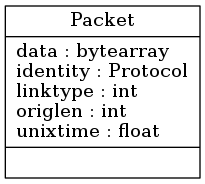
\includegraphics[scale=0.7]{diagrams/packet.png}
\caption{The packet class}
\end{figure}

Here, \emph{linktype} is an integer constant that represents one of many network media types. An important design decision was to make as few assumptions as possible about program input, so this field exists to identify what kind of packet this is. The most common value for this will be $1$, which corresponds to Ethernet (\texttt{LinkType.ETHERNET}) but other values are possible and should be supported.

The \emph{identity} is a field holds the root (i.e. the bottom most) \emph{protocol instance}  for this packet. This should be set to None by default, signifying the packet has not been identified. More on this in the \emph{Protocols} section (\ref{sec:desproto}).

\subsection{Packet Sources and Sinks}
\label{sec:despacksrc}
In order to help ensure scalability, the flow of the system should work around processing individual packets, rather then entire collections of packets. This means a packet is only resident in memory for the time it is needed - permitting processing very large files without too much memory usage. 

\emph{Packet sources} are the realisation of this goal. Packet sources are objects that support Python's \emph{iterator protocol}, that yield the packet objects mentioned in the previous section. Packet sources are presented by the library as building blocks for higher level applications.
Packet sources represent a kind of lazily-evaluated interface towards streams of packets - this cuts down on memory usage, improving scalability. Sources that depend on other sources can be chained without restriction.

A certain type of packet source, a packet reader, is to represent sources based off the various packet capture file formats. These classes implement methods in an abstract class, PacketReader. This abstract class will implement the interface of a packet source using \texttt{read_packet}, and can be used just like one. Along with a packet reader, a packet writer class is available as a \emph{packet sink} - there are no semantics beyond implementing the \texttt{close} and \texttt{write_packet} methods in the PacketWriter class.

\begin{figure}[H]
\center
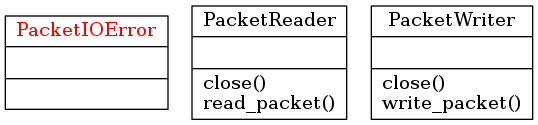
\includegraphics[scale=0.7]{diagrams/packetio.png}
\caption{The PacketReader and PacketWriter abstract classes, with the generic PacketIOError exception.}
\end{figure}

The PacketReader and PacketWriter classes should also raise exceptions when they find a problem reading or writing a packet, respectively. The exceptions raised should be derive from the PacketIOError class.

\subsection{Protocols and Protocol Instances}
\label{sec:desproto}
Network protocols are represented by Protocol classes. Protocols are the most complex abstraction represented in this design.

Logically speaking, instances of communication over a network conform to a linear hierarchy of protocols. A \emph{carrier protocol} encapsulates another protocol, which itself may be another carrier protocol. The system models a packet's identity around the concept of \emph{protocol instances}, which are instances of communication adhering to a specific protocol.

\begin{figure}[H]
\center
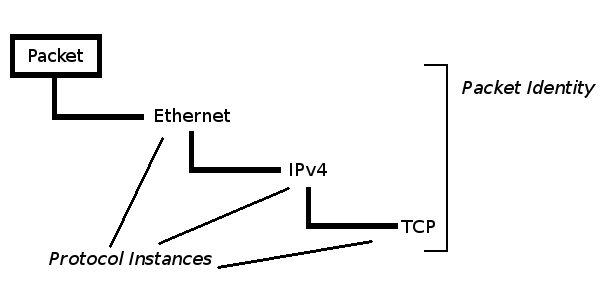
\includegraphics[scale=0.7]{diagrams/protocol-instances.png}
\caption{A packet's identity and protocol instances.}
\end{figure}

A carrier protocol will also have some kind of \emph{route}, a known source and destination. This may or may not depend  on the parent protocol. For instance, IP packets will typically be sent over Ethernet frames, but IP implements a logically independent network from an Ethernet network - these frames, when reaching a router, will be sent somewhere else (with altered frame data), potentially to entirely different routers over an entirely different carrier, all while preserving the IP frame. This is how internetworking works. Conversely, UDP packets rely on the logical route established by IP packets to transmit data, and are basically an extension of the \emph{protocol} or \emph{next} field in an IP header.

\begin{figure}[H]
\center
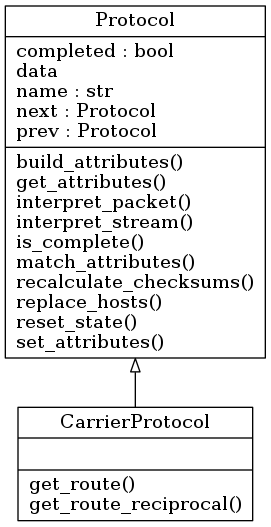
\includegraphics[scale=0.7]{diagrams/protocol.png}
\caption{The protocol and carrier protocol classes}
\end{figure}

The diagram above shows the design of the Protocol and CarrierProtocol classes. For any protocol to be represented in the program, it must have a Protocol class. This class has a well defined form, and this is important as extensibility is a key requirement.

Protocol classes have a single \emph{class variable} and three \emph{unbound methods} (static methods), in addition to the per-instance fields and bound methods typical of most classes. These are used to identify the protocol, and construct \emph{protocol instances} respectively. A more detailed description of these is given below.

Firstly, every protocol instance has a field called data. This is intended to be used as a quasi-internal field, holding either a Python `memoryview' object or a `memorymap' object (see \ref{sec:memmap}). Python \texttt{memoryview} objects are effectively pointers to regions of memory held by objects supporting the \emph{buffer} protocol. A \texttt{memoryview} of a \texttt{bytearray} provides a read-write view of that data without requiring a direct reference to it. Like most python collections, \texttt{memoryview} objects support being sliced - this is important.

Because packets have a linear hierarchy of protocols, Protocol instances have a structure not unlike a linked list - each instance has a parent protocol (called \texttt{prev}) and a child protocol (called \texttt{next}); these are set to none if this is the bottom most or top most protocol, respectively.

Additionally, there is a boolean value called \texttt{completed}, which is to signify whether this protocol instance has finished being dissected. Setting this value to false allows other parts of the code to know that a packet has had its identification deferred until more information is available.

As for bound methods, there are 6 defined, \texttt{get_attributes}, \texttt{set_attributes}, \texttt{match_attributes}, \texttt{is_complete}, \texttt{recalculate_checksums} and \texttt{replace_hosts}.

The \texttt{is_complete}, \texttt{recalculate_checksums} and \texttt{replace_hosts} methods are all propagating methods - they will call their own equivalent on the child protocol instance, if any. \texttt{is_complete} works on the aformentioned \texttt{completed} boolean, returning true if and only if this value is true for all child protocols.

As replacing host identity information is one of the goals of the project, a \texttt{replace_hosts} method was defined. This takes a single argument, a dictionary. This dictionary defines a mapping between host identifiers and their replacements, the idea being that implementations of this method will look for possible substitutions and alter their instance data accordingly, and then call \texttt{replace_hosts} on the child instance. This provides a very simple and reliable way of doing this substitution. In a similar vein, \texttt{recalculate_checksums} is for updating any checksum data. Actual recalculation should start from the top most protocol instance, as the lower level carriers may have checksums on their payload (i.e. UDP).

The \texttt{get_attributes}, \texttt{set_attributes}, \texttt{match_attributes} (and \texttt{build_attributes})  methods all work with or produce  a set of \emph{protocol attributes}. The precise format of said attributes is entirely up to the implementing class, but is suggested to be a \emph{dictionary}.

\texttt{get_attributes} should to return `attributes' of that protocol instance (for example, IPv4 attributes might contain the source/destination address and the protocol number). Conversely, \texttt{set_attributes} should to alter packet data such that the packet corresponds to the attributes provided. \texttt{match_attributes} compares a set of attributes to those of the protocol instance - if they match, this method returns true, else false.

Protocol classes are also required to have a few unbound methods. The most important one, is \texttt{interpret_packet}. 
This method takes two arguments, a \texttt{memoryview} or \texttt{memorymap} object, and a \emph{parent} protocol instance. It is the job of this method to construct and return a protocol instance, possibly calling \texttt{interpret_packet} a subset of the data provided. This method is also responsible for maintaining state for completing deferred identification. \texttt{interpret_stream} effectively does the same thing, but for \emph{streams}.
Because both of these methods may have side effects, as a library, it was deemed appropriate to have some kind of mechanism for restoring the default set of state for these classes - this is the job of the \texttt{reset_state} method.

\texttt{build_attributes} is the last unbound method. This method is intended to return attributes not unlike those returned by \texttt{get_attributes}, and is used for turning human input (an `attribute string') into a workable object.

Finally, all protocol classes need to have a human-readable name. This is for both output (such as when `printing' a packet) but mainly as a unique identifier for a Protocol class. The intention is, that protocols are referred to by this name, and that a Protocol class can be replaced by one with the same name, should the user want to use an alternate implementation. This name is also used in constructing and comparing attributes.

\pagebreak
\section{Memory maps}
\label{sec:memmap}
In order to identify protocols, packet data needs to be examined. As some protocols can have a variety of carriers, and carrier protocols can have a variable size, the exact location of one protocol's header is not a constant offset.

The initial approach to this problem was just to copy the payload section of a protocol and present that to the next protocol interpreter. This works, but means any modifications to the protocol header would require the entire packet to be rebuilt - a time consuming operation.

Python \emph{memoryview} objects provide a memory-efficient and simple way of presenting smaller sections of data from an object. They are probably best illustrated with an example:
\begin{lstlisting}[
	language={[3]Python},
   	caption={[Memoryview demonstration]A demonstration of memoryviews. v is a view of data, and v1/v2 are subviews of data.}
]
>>> data = bytearray(b"abcdef")
>>> v = memoryview(data)
>>> bytes(v)
b'abcdef'
>>> v1 = v[0:3]
>>> v2 = v[3:6]
>>> bytes(v1)
b'abc'
>>> bytes(v2)
b'def'
>>> v2[1] = b"E"
>>> bytes(v)
b'abcdEf'
\end{lstlisting}
Here, some data object (called \texttt{data}) is being read and altered by some \emph{memoryview} objects (called \texttt{v}, \texttt{v1} and \texttt{v2}).

Importantly for this project, alterations to \emph{memoryview} objects affect their backing store - changes are reflected in the object the views are based on. These are sufficient to provide a linear tree of protocol instances with read/write access to packet data, but it was known from the start of the project that sometimes, parts of protocol data will exist over many packets.

For identification purposes, this can easily be solved by simply copying parts of the fragmented data and concatenating them. This solution is a different application of the first solution presented and suffers from all its downsides in addition to the problem of making alteration a very difficult task.

To solve this problem efficiently, a \emph{memorymap} class is needed. This class would provide logically contiguous access to multiple, separate \emph{memoryview} objects.

The ideal implementation would have a similar interface to that of \emph{memoryview} objects, and function as a drop-in replacement. This means protocol classes need not worry over how many packets their data is spread.

\section{User Interface}
The project is more then just a library. The project also seeks to provide a useful user interface to manipulate packet captures. In terms of requirements, this section refers to the design of \ref{fr:6} \emph{merge program}. \ref{fr:7} \emph{timestamp alteration program}, \ref{fr:8} \emph{filter program} and \ref{fr:9} \emph{host identity replacement program}.

As is normal for batch data processing tools, these have a command line interface.

\subsection{Common interface elements}
The programs are to understand their command line arguments as a series of options with mostly unary or nullary parameters. For ease of use, there will be no specific order to command line options and no explicit options will be mandatory, each program having \emph{default} behaviour.

Here, arity means how many arguments the option requires, i.e. a nullary option takes no arguments,  a unary option requires one, a binary option would require 2 etc.
Frequency is how often the option should appear. Singular indicates the option should appear at most once, arbitrary means the option can appear any number of times.

There will be commonalities between tools. These are detailed below.

\begin{tabularx}{\textwidth}{|c|c|c|c|X|}
\cline{1-2}
\multicolumn{2}{|c|}{\textbf{Option Flag}} & \multicolumn{3}{c}{}\\ \hline
\textbf{Short} & \textbf{Long} & \textbf{Arity} & \textbf{Frequency} & \textbf{Description} \\ \hline
\texttt{-l} & \texttt{--load} & unary & arbitrary & Loads a external support code module.\\ \hline
\texttt{-h} & \texttt{--help} & nullary & singular & Prints out help text.\\\hline
\texttt{-i} & \texttt{--input} & unary & singular & The capture file to read from (defaults to stdin).\\ \hline
\texttt{-o} & \texttt{--output} & unary & singular & The capture file to write to (defaults to stdout).\\ \hline
\end{tabularx}

\subsection{The List Tool}
\label{sec:listdes}
The list tool will take a packet capture, and print out a succinct, human-readable interpretation of each packet.

The list tool has no special parameters, and does \emph{not} accept the \texttt{--output} option.

The output should be something along the lines of:

{\small\texttt{Mon Oct 20 15:51:29 2014 Linktype: 1, Identity: eth/arp, Length: 42}}

\subsection{The Merge Tool}
\label{sec:mergedes}
The merge tool will take an arbitrary number of packet capture files, and write out a single capture from these.

The merge tool was also seen as the appropriate place to do time alteration, so this program fulfils the role of \ref{fr:6} \emph{merge program} and \ref{fr:7} \emph{timestamp alteration program}.

The merge tool will take a slightly different \texttt{--input} option in that it will permit the option to occur multiple times.

\begin{tabularx}{\textwidth}{|c|c|c|c|X|}
\cline{1-2}
\multicolumn{2}{|c|}{\textbf{Option Flag}} & \multicolumn{3}{c}{}\\ \hline
\textbf{Short} & \textbf{Long} & \textbf{Arity} & \textbf{Frequency} & \textbf{Description} \\ \hline
\texttt{-i} & \texttt{--input} & unary & arbitrary & The capture files to read from (if none specified, reads from stdin exclusively).\\ \hline
\texttt{-r} & \texttt{--relative} & nullary & singular & Makes all packet arrival times from a file relative to the time the first packet recorded in that file (this is on by default).\\ \hline
\texttt{-a} & \texttt{--absolute} & nullary & singular & Packets retain their original time (this is the opposite of the \emph{relative} mode above).\\ \hline
\texttt{-t} & \texttt{--offset} & unary & singular & Time offset, this value is added to the arrival times of all packets. If this value is not provided, it is set to the \emph{average arrival time of the first packet in each capture}. \\ \hline
\end{tabularx}

\begin{verbatim}
[user@host ~]$ merge -i cap1.pcap -i cap2.pcap -o cap12.pcap
\end{verbatim}

\subsection{The Filter Tool}
\label{sec:filterdes}
The filter tool will fulfil the role of \ref{fr:8} \emph{filter program}.

\begin{tabularx}{\textwidth}{|c|c|c|c|X|}
\cline{1-2}
\multicolumn{2}{|c|}{\textbf{Option Flag}} & \multicolumn{3}{c}{}\\ \hline
\textbf{Short} & \textbf{Long} & \textbf{Arity} & \textbf{Frequency} & \textbf{Description} \\ \hline
\texttt{-k} & \texttt{--keep} & unary & arbitrary & A packet identity to keep.\\ \hline
\texttt{-d} & \texttt{--discard} & unary & arbitrary & A packet identity to discard.\\ \hline
\texttt{-p} & \texttt{--policy} & unary & singular & The policy to apply to any unaccounted for packet. Accepts either \emph{keep} or \emph{discard}.\\ \hline
\end{tabularx}

The tool will operate by first checking if a packet's identity matches anything in the \emph{keep} set. If so, the packet will be reproduced in output. If not in the \emph{keep} set, the packet's identity is then checked against items in the \emph{discard} set. If any match is sound, the packet will not be present in output. If a packet's identity is not present in either set, the value of \emph{policy} is used - if keep, the packet is kept, if discard, the packet is discarded.

Here, an \emph{identity} will be specified as a specially formatted string, consisting of \emph{protocol names} and \emph{protocol attributes}.

Valid protocol names are arbitrary strings\footnote{In the case of protocol names, ideally alphanumeric.} that contain no colons or slashes. Valid protocol attributes share the same restrictions.

\begin{grammar}
<prototype> ::= <protocol name> `:' <protocol attributes>
\alt <protocol name>

<identity> ::= <prototype> | <prototype> `/' <identity>
\end{grammar}

The exact format of the protocol attributes string depends entirely on the Protocol class, this string will be parsed by the \texttt{build_attributes} method. However, a consistent format should be used (but not imposed) - to this end, the format used by all built-in Protocol classes will take the form of a simple key-equals-value semicolon separated list.

\begin{grammar}
<kvp> ::= <key> `=' <value>

<protocol attributes> ::= <kvp> | <kvp> `;' <protocol attributes>
\end{grammar}

Invocation might look like:

\begin{verbatim}
[user@host ~]$ filter -i cap1.pcap -o cap1-noip6.pcap -k eth/ip6 -p discard
\end{verbatim}
for permitting only IPv6 packets, or

\begin{verbatim}
[user@host ~]$ filter -i cap1.pcap -o cap12.pcap -d eth/arp:opcode=1
\end{verbatim}

for removing all ARP requests, leaving ARP responses intact.

\pagebreak
\subsection{The Maphosts Tool}
\label{sec:maphostsdes}
The `maphosts' realises \ref{fr:9} \emph{host identity replacement program}.

\begin{tabularx}{\textwidth}{|c|c|c|c|X|}
\cline{1-2}
\multicolumn{2}{|c|}{\textbf{Option Flag}} & \multicolumn{3}{c}{}\\ \hline
\textbf{Short} & \textbf{Long} & \textbf{Arity} & \textbf{Frequency} & \textbf{Description} \\ \hline
\texttt{-m} & \texttt{--mac} & unary & arbitrary & A mapping of an Ethernet MAC address to its replacement.\\ \hline
\texttt{-4} & \texttt{--ip4} & unary & arbitrary & A mapping of an IPv4 address to its replacement.\\ \hline
\texttt{-6} & \texttt{--ip6} & unary & arbitrary & A mapping of an IPv6 address to its replacement.\\ \hline
\end{tabularx}

The \texttt{-m}, \texttt{-4} and \texttt{-6} understand address pairs as their argument. Address pairs have the form:

\begin{grammar}
<address pair> ::= <address> `=' <address>
\end{grammar}

The address here, will take the form:

\begin{grammar}
<hexbyte> ::= 00 | 01 | 02 | 03 ... FF

<hexpair> ::= <hexbyte> <hexbyte>

<decbyte> ::= 0 | 1 | 2 | 3 ... 255

<MAC address> ::= <hexbyte> `:' <hexbyte> `:' <hexbyte> `:' <hexbyte> `:' <hexbyte> `:' <hexbyte>

<IPv4 address> ::= <decbyte> `.' <decbyte> `.' <decbyte> `.' <decbyte>

<IPv6 address> ::= <hexpair> | <hexpair> `:' <IPv6 address>
\alt <IPv6 address> `::' <IPv6 address>
\end{grammar}

Note that this particular grammar definition of an IPv6 address is rather vague. A more detailed explanation is given in RFC 5952\cite{rfc5952}.

Typical invocation might be:

\begin{verbatim}
[user@host ~]$ maphosts -i cap1.pcap -o cap12.pcap -4 192.168.0.20=172.16.0.20
\end{verbatim}

for replacing occurences of \texttt{192.168.0.20} with \texttt{172.16.0.20}.

\chapter{Implementation}
Implementation started concurrently with design. Challenges encountered during implementation would change the design, and vice versa.

Due to the sheer number of networked protocols and the complexities in supporting some of them, the project was never expected to approach $100\%$ completion. As a result of this, much of the implementation time was actually spent improving the design sufficiently to correctly support a small subset of protocols, while considering other protocols being added in the future.

An interesting point to note is that no external\footnote{External dependencies being anything not present in the Python standard library.} dependencies or code were used. Only builtin Python classes and modules in the standard library were used. These were the \texttt{struct} module,  the \texttt{sys} module, the \texttt{binascii} module and (for the commandline interface, the \texttt{argparse} module).

The source code to the project may be found on the additional media supplied with this document, if this is a physical copy.

\section{Meta-Implementation}
While this section is not really about any specific implementation detail, it does cover noteworthy disciplines used by the author \emph{while implementing}.

\subsection{Coding Style}
Some of the functional requirements (namely \ref{nfr:10} \emph{code structure} and \ref{nfr:11} \emph{code documentation}) effectively require code to be well-written and well-documented.

To this end, a variant of the standard Python code style was used. In essence:
\begin{enumerate}[label=\roman*)]
\item Indentation is done with four spaces.\\
\item \emph{Private} fields in a class start with an underscore.\\
\item Functions and methods are lower\textunderscore{}case\textunderscore{}with\textunderscore{}underscores.\\
\item Constants are CAPITALS\textunderscore{}WITH\textunderscore{}UNDERSCORES.\\
\item Class identifieirs are written in UpperCamelCase.
\end{enumerate}

In contrast to normal Python style guidelines, this particular style makes classes easy to differentiate from functions.

In addition to following the aforementioned coding style, the code was also written to be mostly PEP8\cite{pep8} compliant (this was checked with the \texttt{pep8} conformance checker, see \cite{pep8chk}).

\subsection{Version Control}
Any programming project will benefit form a form of version control. Version control helps keep a record of progress and allows mistakes to be easily reverted.

Version control is also useful as a kind of synchronisation system between multiple computers, permitting an individual to continue work while away from their normal work environment.

The author used \emph{git} (\url{http://git-scm.com}) as the version control system (VCS), due to having prior knowledge on how to use it.

\section{The \texttt{packet} super-package}
The `library' portion of the implementation is contained within its own package, the \texttt{packet} package. All of the modules have PyDoc docstrings, allowing for interactive documentation browsing with the pydoc utility. Should the reader want to do this, simply do:

\texttt{\$ pydoc -b packet}

from the \texttt{src} directory. The same documentation is also included in the appendix (section \ref{sec:apidoc}).

\section{The \texttt{memorymap} Module}
The \texttt{memorymap} module implements the \emph{memorymap} class as described in \ref{sec:memmap}, and works by mapping multiple \emph{memoryview} objects to a single \emph{logical} `index space'.

The \texttt{memorymap} class stores each constituent \emph{memoryview} object (denoted $V$) as part of a three-tuple,  with their \emph{logical} starting and ending index ($min$ and $max$, respectively). This tuple is henceforth referred to as a \emph{segment} (or $S$). These segments are stored in a list ($Q$), in ascending order of ranges.

{\small
A note on notation: Slightly non-standard notation and concepts have been employed to make this mathematical model more readable and understandable. \emph{Lists} are \emph{tuples} with different notation.

For a tuple, superscript denotes a component, i.e.  for tuple $T = (a,\, b,\, c\, ...)$,   $T^{a} = a$.

For a list, square brackets denote a specific element, i.e. for list $R = (\pi,\, \epsilon,\, \lambda\, ...)$, $R[3] = \lambda$
}

\begin{align*}
S_{i} &= ( V_{i},\, min_{i},\, max_{i} )\\
Q &= [ S_{0},\, S_{1},\, S_{2}\, ... \,S_{i} ]\\
\end{align*}
\begin{center}
Given $S_{a}$ and $S_{b}$ as any two elements in $Q$, where $a < b$,
\end{center}
\begin{align*}
&\ S_{a}^{max} \leq S_{b}^{min} 
\end{align*}

A \emph{logical index} ($n_{logical}$) is translated to a pair of actual indices, the \emph{segment index} ($n_{segment}$), which refers to one of the segments in the segment list, and a \emph{local index} ($n_{local}$), which is the part of the segment.

This translation is done by a very simple algorithm. A binary search of the segment list is done, identifying the range encompassing a \emph{logical index}.

\begin{align*}
n_{segment} &= search(Q,\,n_{logical})\\
N &= Q[n_{segment}]\\
n_{local} &= n_{logical} - N^{min}
\end{align*}

\section{The \texttt{common} Module}
The common module contains functions and classes which are useful in many different locations.
This is where the packet class is defined.

This class contains the rather large \texttt{LinkType} enumeration, used in the identity package and the capfile package.

Also contained, is a handful of input parsing functions. A few basic ones, such as \texttt{parse_int} and \texttt{parse_hexbytes}.

There are functions for parsing string representations of MAC, IPv4 and IPv6 addresses, and turning binary representations into strings. these are named \texttt{*_str2bin} and \texttt{*_bin2str}, and take a single argument returning None if the format is erroneous.

\section{The \texttt{capfile} Package}
This package contains code for reading and writing abstract packets to packet capture files. Currently, only the \emph{pcap} files are supported, but the author hopes that extending the library and programs to accept different formats to be relatively straightforward.
 
\subsection{The \texttt{core} Module}
This contains abstract classes intended to make adding new capture formats easier. Very simple PacketReader and PacketWriter classes are provided, with a PacketIOError exception class for abstracted error handling.

\subsection{The \texttt{pcap} Module}
This module contains two classes, a PcapReader class, which implements abstract methods in the PacketReader class, and a PcapWriter class, which implements abstract methods in the PacketWriter class.

These classes implement support for manipulating \emph{pcap} files according to the pcap format specification\cite{pcapfmt}, which is described below.

\begin{figure}[H]
\center
\begin{bytefield}{32}
\bitheader{0-31}\\
\wordbox{1}{Magic Number}\\
\bitbox{16}{Version Major} & \bitbox{16}{Version Minor}\\
\wordbox{1}{Time Zone Offset}\\
\wordbox{1}{No. of Significant Figures}\\
\wordbox{1}{Maximum Snapshot Length}\\
\wordbox{1}{Linktype}
\end{bytefield}
\caption{pcap global header.}
\label{fig:pcapglob}
\end{figure}

The pcap format is quite simple, perhaps the reason for its ubiquity. A pcap file starts with a \emph{magic number} field. This indicates the format specifics of that capture file. The magic number is $a1\: b2\: c3\: d4$ for \emph{millisecond resolution} pcap files, and $a1\: b2\: 3c\: 4d$ for \emph{nanosecond resolution} files. Additionally, this field is in the same byte ordering as the rest of the fields in the file, so $d4\: c3\: b2\: a1$ would indicate that the file stores little-endian millisecond resolution fields, rather then big-endian.

The rest of the fields are indicated in figure \ref{fig:pcapglob}, and are fairly self explanatory. Linktype is an integer constant indicating the network media (such as Ethernet). These are the same as the values present in the \texttt{common} module.

\begin{figure}[H]
\center
\begin{bytefield}{32}
\bitheader{0-31}\\
\wordbox{1}{Timestamp (seconds)}\\
\wordbox{1}{Timestamp (milli/nanoseconds)}\\
\wordbox{1}{Recorded Snapshot Length}\\
\wordbox{1}{Original Snapshot Length}
\end{bytefield}
\caption{pcap record header}
\label{fig:pcaprec}
\end{figure}

Pcap \emph{records} consist of a record header and a packet snapshot. The packet data is presented verbatim, as it was on the network, but truncated to fit within the maximum snapshot length defined in the header.

The record header also has a simple layout. A 32-bit timestamp, in seconds since the UNIX epoch, and another 32-bit field of either millisecond or nanosecond resolution time, which serves as additional precision for this value.

Two more 32-bit fields are present, consisting of the recorded snapshot length and the original snapshot length. The recorded length indicates how many bytes after this header belong to a packet snapshot. Record headers immediately follow the global header and snapshot data.

These classes handle erroneous data in a robust and well defined manner - if the PcapReader encounters a truncated file, it will read and return all entries which are intact, raising a PcapFormatError exception when the truncated entry is reached.
 
If the PcapWriter is instructed to write a packet with a LinkType that differs from that of the network section of the file, it will raise a PcapRangeError exception.

\section{The \texttt{identity} Package}
This module is where most of the interesting code is and is the package where all `builtin' protocol classes reside.

\subsection{The \texttt{core} Module}
The core module in the identity package is where the Protocol class is defined. This serves as step 0 in the packet identification system.

This module contains the registry of all supported protocols, and maintains a mapping of \emph{protocol name} to \emph{protocol class}. All Protocol classes should be registered with this module. Additionally, this module maintains a mapping of \emph{linktypes} to \emph{protocol names}, used in order to determine  which \emph{base protocol class} to use.

The Protocol registration and resolution is done using the \texttt{register_protocol} and \texttt{lookup_protocol}. The use of a string identifier instead of a direct class reference serves two purposes: Firstly, it allows for \emph{alternate} implementations of builtin Protocol classes to be used, and provides an easy way for parts a program, particularly those that handle user input, to get access to the same Protocol class used in the identity of a packet.

More importantly, it provides the \texttt{root_identify} function, which starts the identification of a packet. This function does not pay attention to \emph{deferred} identities, so applications that want a more complete understanding of packets should use the \texttt{identify} pipeline instead.
 
\subsection{The \texttt{ip} Module}
The \texttt{ip} module is part of the identity package, and is used by the the \texttt{ip4} and \texttt{ip6} modules.

The \texttt{ip} module provides a registry of Protocol classes mapped to IP protocol numbers. It also contains a handful of constants for said numbers\footnote{see IANA for a complete list, \url{http://www.iana.org/assignments/protocol-numbers/protocol-numbers.xhtml}}. Registration is done just as in the \texttt{core} module.

Aside from providing the IP protocol registry used by these modules, it provides an implementation of the checksum algorithm mentioned in \ref{sec:ip4}. This is used by the IPv4, TCP and UDP Protocol classes, and should be sufficient for others using similar schemes.
\begin{lstlisting}[
	language={[3]Python},label={lst:pyipchksum},
	caption={IP checksum algorithm, in Python.}
]
# The checksum algorithm is:
#      The checksum field is the 16 bit one's complement of the one's
#      complement sum of all 16 bit words in the header.  For purposes of
#      computing the checksum, the value of the checksum field is zero.

def checksum(data):
    # General implementation of the IP checksum algorithm.
    n16words, rem = divmod(len(data), 2)

    if rem != 0:
        # Argument is not in terms of 16-bit words.
        return None

    # generate list of 16-bit words.
    words = [word for word in struct.Struct("!"+"H"*n16words).unpack(data)]

    ocsum = 0
    for word in words:
        # One's complement addition of 16-bit words.
        acc = ocsum + word
        carry = acc >> 16
        ocsum = (acc + carry) & 0xFFFF

    b1, b2 = divmod(ocsum, 256)
    return bytes((~b1 & 0xFF, ~b2 & 0xFF))
\end{lstlisting}

\subsection{The Protocol classes}
There are quite a few Protocol classes implemented, enough to provide basic sanitisation and anonymisation features useful for the project.

In this project, each protocol class has its own Python module. The modules that currently exist are \texttt{eth}, \texttt{arp}, \texttt{ip4}, \texttt{ip6}, \texttt{tcp} and \texttt{udp}, \texttt{icmp} and \texttt{icmp6}. (Albeit some are incomplete, see the critical evaluation in chapter \ref{sec:criteval}).

All of these classes expose the same interface as specified in section \ref{sec:desproto} of the design chapter. Because there are so many, this section will focus on one, the IPv4 class in the \texttt{ip4} module.

The IPv4 class is one of the more complex Protocol classes, namely because it specifies fragmentation behaviour and has a checksum.

Internally, the IPv4 class makes use of a `\texttt{FragmentTracker}' class. This class exists to store references to all packets that make up a fragmented datagram. Until such a packet is complete, the \texttt{completed} boolean field is set to false for all constituents. Once the composite datagram is known to be complete, the \texttt{completed} field is set to true, a \texttt{memorymap} is created from the payloads of all constituent packets, and presented to the next Protocol class.

Once a complete datagram is reassembled, the protocol field in the IP header (see figure \ref{fig:ip4fmt}) is used with the \texttt{ip.lookup_ip_protocol} function to determine the next Protocol class to use. The \texttt{next} field for all constituent IPv4 instances is set to that of the new Protocol class and the \emph{last} fragment becomes the parent for that class.

\section{The \texttt{pipeline} Package}
The pipeline package provides three packet sources, \texttt{merge}, \texttt{filter} and \texttt{identify}.
These all behave like packet sources as described in \ref{sec:despacksrc}, and accept packet sources as input.

\subsection{The \texttt{merge} Module}
The \texttt{merge} module contains the \emph{merge} generator function.

This function takes a list of packet sources and two optional parameters, \emph{relative} and \emph{offset}.
If relative is true, then the time stamp of the first packet from a source is subtracted from all packets from that source.
If offset is set to any number, this value is added to the time of all packets, otherwise the average start time is used in place. This function returns a generator that produces the next chronological packet on each iteration.

\subsection{The \texttt{filter} Module}
The \texttt{filter} module contains the \emph{filter} generator function.

The filter function takes a packet source, two sets of \emph{prototype lists} and a policy.

A prototype list is simply a list of \emph{prototypes}. A prototype is a 2-tuple, consisting of a protocol name and a set of protocol attributes. These protocol attributes are usually obtained from the \texttt{build_attributes} static method in the Protocol class with the corresponding name.

A prototype list matches a protocol identity if:
\begin{enumerate}[label=\roman*)]
\item Each prototype in the prototype list has a protocol name matching that of the corresponding protocol instance in the identity.
\item Each prototype in the prototype list has a set of protocol attributes which, when passed to the \texttt{match_attributes} method of the corresponding protocol instance, evaluates to true.
\item The number of protocol instances in the protocol identity is equal to or greater than the number of prototypes in the prototype list.
\end{enumerate}

There is an internal function, \texttt{identity_match}, that implements the matching algorithm described above.

\begin{lstlisting}[
	language={[3]Python},label={lst:identmatch},
	caption={Packet identity matching algorithm.}
]
def identity_match(protocol_instances, prototypes):
    # Compares a packet's identity list (protocol instances) to a list of
    # 'prototypes'.
    # Every prototype must match it's corresponding protocol instance.
    # Prototypes are a (name, attrs) tuple.
    
    prototype_iter = iter(prototypes)
    match = False
    for protocol_instance, prototype in\
      zip(protocol_instances, prototype_iter):
        if protocol_instance.name is not prototype[0] or \
          not protocol_instance.match_attributes(prototype[1]):
            break
    else:
        # This checks if the number of prototypes exceeds
        # the number of protocol_instances.
        try:
            next(prototype_iter)
        except StopIteration:
            match = True

    return match
\end{lstlisting}

These two sets of prototype lists are the \emph{keep} set and \emph{discard} set.
Any packet matching something in the keep set is remitted as output, any packet matching something in the discard set is not. If a packet matches no prototype lists, the \emph{policy} is used, either keeping or discarding the packet.

\subsection{The \texttt{identify} Module}
The \texttt{identify} module contains the \emph{identify} generator function.

This function is very simple, and offers a nicer interface to the \texttt{root_identify} function in the \texttt{identity.core} module.

For every packet in the provided source, it will pass it to the \texttt{root_identify} function. If the identity is incomplete, it will store the packet in a buffer and read the \emph{next} packet, buffering these until the first packet has it's identity completed.

If the packet source is exhausted before a packet has its identity completed, then the incompletely identified packets are returned.

\section{The \texttt{pcpapu} Tool}
During development, it was deemed easier to implement the utilities as \emph{subcommands} in a larger utility.

PCPAPU stands for `Packet Capture Processor and Publishing Utility', and at its basic level, implements the \texttt{-l} option, and provides a rudimentary way of loading support code.

This utility comes with seperate help text for all subcommands, see appendix (section \ref{sec:helptext}).

\subsection{The \texttt{list} Subcommand}
The list subcommand implements the same interface as that of the list tool described in the design section \ref{sec:listdes}.

The list command is a very simple tool. Input parsing aside, the list tool consists of a rather elegant two lines:
\begin{lstlisting}[
	language={[3]Python},label={lst:listimp},
	caption={Important section of the list tool.}
]
for packet in identify(source):
    print(packet)
\end{lstlisting}

\subsection{The \texttt{merge} Subcommand}
The merge subcommand implements the same interface as that of the merge tool described in the design section \ref{sec:mergedes}.

The merge subcommand exposes the same interface as the merge pipeline. Its input processing expects a date in a specific form, \texttt{YYYY/MM/DD HH:MM:SS}, which is converted into a UNIX timestamp.

Note that this does make for some rather non-intuitive behaviour. In order to merge capture files without altering their timestamps, it is necessary to specify ``\texttt{1970/1/1 00:00:00}'' as the time offset in addition to specifying the \texttt{-a} flag. This interaction should be reviewed at a later date.

\subsection{The \texttt{filter} Subcommand}
The filter subcommand implements the same interface as that of the filter tool described in the design section \ref{sec:filterdes}.

Just like the merge subcommand, this is implemented in terms of \emph{pipelines}, first using the identify pipeline, then the filter pipeline.

\subsection{The \texttt{maphosts} Subcommand}
The maphosts subcommand implements the same interface as that of the maphosts tool described in the design section \ref{sec:maphostsdes}.

It utilises the identify pipeline, and will call the cascading \texttt{replace_hosts} method and \texttt{recalculate_checksums} method on the root protocol instance for each packet.

\chapter{Testing}
The testing for this project was done throughout development. 
A rather informal mixture of \emph{white box} and \emph{black box} testing was employed throughout most of the development process. Typically, a small test run with known inputs and expected outputs was run after every major feature or re-factoring work was carrier out, and if erroneous or regressive behaviour was observed, code was reviewed and debugged.

\section{Testing During Development}
During development, a straightforward develop-test-debug approach was used to check for correctness in new code. Any newly implemented feature would be tested.

For simple modules, an interactive Python interpreter was started and the module imported and interacted with. Many errors in early modules were detected this way.

\begin{figure}[H]
\center
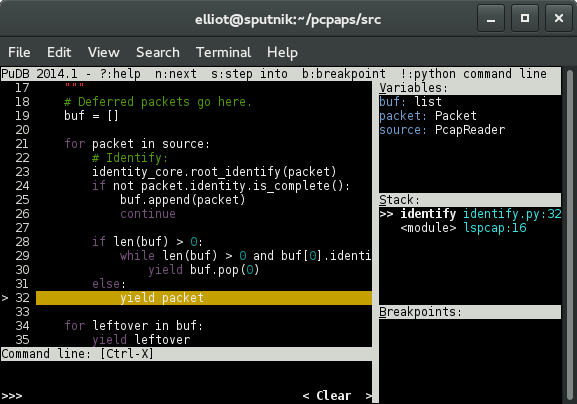
\includegraphics[scale=0.75]{pictures/pudb.png}
\caption{Screenshot of pudb, the debugger used. (\url{http://pypi.python.org/pypi/pudb})}
\end{figure}

When the programs became more complex, a debugger was used. This permitted analysis of complex state at runtime without the (mis)use of `print statements'.

\subsection{Regression Testing}
When any major feature stopped working, the use of version control and the regression itself (altered output, stack traces etc.) made it easy to determine what changes had caused the problem, and made fixing it simple.

Explicit regression testing was done whenever any code re-factoring was carried out.

\subsection{Output verification}
Output was generally verified using \emph{Wireshark}, to see if the output was a valid pcap file and if packet data was modified correctly. Features of Wireshark such as checksum verification were employed to test wheter checksum recalculation algorithms worked.

\section{Black-Box Testing}
For these tests, a real network capture between two computers, containing examples of various protocols (in excess of the ones supported) was used. This packet capture starts from 2014/10/20 at 15:49:59.

\subsection{Testing the List Tool}
The list tool is a very straightforward tool, and was used mostly to verify the output of other tools. Nevertheless, this tool represents a kind of benchmark - if this tool does not work correctly, none of the others are likely to function.

\begin{tabularx}{\textwidth}{|c|X|X|X|X|}
\hline
\textbf{Test} & \textbf{Input} & \textbf{Expected} & \textbf{Actual} & \textbf{Comments}\\
\textbf{ID} & & \textbf{Output} & \textbf{Output} &
\endhead
\hline
LIS1 & filepath specified with the \texttt{-i} option & Listing of packets. & Listing of packets. & Works as expected \\ \hline
LIS2 & capture file piped to standard input & Listing of packets. & Listing of packets. & Works as expected \\ \hline
\end{tabularx}

The exact output of this program was cross-referenced with that of \emph{Wireshark}, with which it agreed with for all supported protocols.

\subsection{Testing the Merge Tool}

To verify the output of these tests, the \emph{list} tool as tested above was used.

\begin{tabularx}{\textwidth}{|c|X|X|X|X|}
\hline
\textbf{Test} & \textbf{Input} & \textbf{Expected} & \textbf{Actual} & \textbf{Comments}\\
\textbf{ID} & & \textbf{Output} & \textbf{Output} &
\endhead
\hline
MER1 & filepath specified with the \texttt{-i} option, different filepath specified with the \texttt{-o} option. &
	A duplicate of the capture file. &
	Almost a duplicate of the capture file. &
	See section \ref{sec:intrsnaplen}. \\ \hline
MER2 & like above, with the \texttt{-t} option set to \texttt{"1970/1/1 00:00:00"} &
	Capture file claiming to start from the 1st of January, 1970. &
	Capture file claiming to start from the 1st of January, 1970. &
	Works as expected \\ \hline
MER3 & like above, with the \texttt{-t} option set to \texttt{"2014/10/30 15:49:59"} &
	Capture file claiming to start from the 30th of October, 2014. &
	Capture file claiming to start from the 30th of October, 2014. &
	Works as expected \\ \hline
MER4 & Two files specified with \texttt{-i}, the other file being the result of the previous test. &
	Capture file consisting of packets interleaved from each file, claiming to start from the 15th of October, 2014. &
	Capture file consisting of packets interleaved from each file, claiming to start from the 15th of October, 2014. &
	Works as expected \\ \hline
MER5 & The \texttt{-a} option enabled and the \texttt{-t} option set to \texttt{"1970/1/1 00:00:00"}, along with two files specified with \texttt{-i}, the other file being the result of MER3. &
	Capture file consisting of packets from each file neatly concatenated, claiming to start from the 10th of October, 2014. &
	Capture file consisting of packets from each file neatly concatenated, claiming to start from the 10th of October, 2014. &
	Works as expected \\ \hline
\end{tabularx}

These captures were also opened in \emph{Wireshark}, which reported no abnormalities.

\subsection{Testing the Filter Tool}
Thorough testing for this for the filter tool would require testing all possible Protocol classes. This would require a lot of time, so testing will focus on demonstrating tool usage scenarios using different protocol classes.

Additionally, not all protocols are supported by the library. \emph{Unsupported} protocols are not identified, and packets that contain them will have a short identity chain, e.g. ``eth/ip4".

\begin{tabularx}{\textwidth}{|c|X|X|X|X|}
\hline
\textbf{Test} & \textbf{Input} & \textbf{Expected} & \textbf{Actual} & \textbf{Comments}\\
\textbf{ID} & & \textbf{Output} & \textbf{Output} &
\endhead
\hline
FIL1 & filepath specified with the \texttt{-i} option, different filepath specified with the \texttt{-o} option. &
	A duplicate of the capture file. &
	Almost a duplicate of the capture file. &
	See section \ref{sec:intrsnaplen}. \\ \hline
FIL2 & As above, but with the \texttt{-d} option given \texttt{eth/arp} as an argument. &
	A similar capture file, stripped of all Ethernet/ARP packets. &
	A similar capture file, stripped of all Ethernet/ARP packets. &
	Works as expected. \\ \hline
FIL3 & As above, but using \texttt{-k} instead of \texttt{-d} and with {-p} set to \texttt{discard} &
	A capture file, containing nothing but Ethernet/ARP packets. &
	A capture file, containing nothing but Ethernet/ARP packets. &
	Works as expected. \\ \hline
FIL4 & Similar I/O flags, with \texttt{-k eth/ip4/tcp} and \texttt{-d eth/ip4} &
	A similar capture file, where all Ethernet/IPv4 packets are removed unless they carry TCP. &
	A similar capture file, where all Ethernet/IPv4 packets are removed unless they carry TCP, or use an unsupported protocol on top of IP. &
	This was discovered to be a bug in the filter pipeline, where more specific prototypes would apparently match less specific identities. \\ \hline
FIL4 & Similar I/O flags, with \texttt{-k eth/ip4/tcp} and \texttt{-d eth/ip4} &
	A similar capture file, where all Ethernet/IPv4 packets are removed unless they carry TCP. &
	A similar capture file, where all Ethernet/IPv4 packets are removed unless they carry TCP. &
	Works as expected, error in filter pipeline fixed. \\ \hline
\end{tabularx}

The filter program performed its job admirably, with only one error corrected in testing.

\subsection{Testing the Maphosts Tool}
Replacement is only expected to function for the protocols supported. This meant that occurrences in unsupported protocols such as DNS are \emph{not} expected to be replaced.

\begin{tabularx}{\textwidth}{|c|X|X|X|X|}
\hline
\textbf{Test} & \textbf{Input} & \textbf{Expected} & \textbf{Actual} & \textbf{Comments}\\
\textbf{ID} & & \textbf{Output} & \textbf{Output} &
\endhead
\hline
FIL1 & filepath specified with the \texttt{-i} option, different filepath specified with the \texttt{-o} option. &
	A duplicate of the capture file. &
	Almost a duplicate of the capture file, with some TCP checksums corrected. &
	See extended commentary in section \ref{sec:tcpchksum}. \\ \hline
FIL2 & Similar, with the addition of \texttt{-m de:ad:be:ef:13:37 = bc:ee:7b:df:e8:08} &
	A variant of the capture file, with all references to the MAC address \texttt{de:ad:be:ef:13:37} replaced with \texttt{bc:ee:7b:df:e8:08}. &
	A variant of the capture file, with all references to the MAC address \texttt{de:ad:be:ef:13:37} replaced with \texttt{bc:ee:7b:df:e8:08}. &
	Worked as expected. References to the old MAC address persisted in the form of link-local IPv6 address. This is not considered a bug\footnote{To elaborate, IPv6 link local addresses are often based on the MAC address of the link hardware they are set on. These addresses are actually IPv6 addresses, and hence should \emph{not} be replaced as a MAC address.}.\\ \hline
FIL3 & Similar, but with \texttt{-4 10.128.128.1 = 192.168.0.20} &
	A variant of the capture file, with all references to the IP address \texttt{10.128.128.1} replaced with \texttt{192.168.0.20}. &
	A variant of the capture file, with all references to the IP address \texttt{10.128.128.1} replaced with \texttt{192.168.0.20}. &
	Works as expected. \\ \hline
FIL4 & Similar, but with \texttt{-6 fe80::14fa:1cff: feaa:7cfa = fe80::f00f:bad0} &
	A variant of the capture file, with all references to the IP address \texttt{fe80::14fa:1cff: feaa:7cfa} replaced with \texttt{fe80::f00f:bad0}. &
	A variant of the capture file, with all references to the IP address \texttt{fe80::14fa:1cff: feaa:7cfa} replaced with \texttt{fe80::f00f:bad0}. &
	Works as expected. \\ \hline
\end{tabularx}

\section{Interesting results}
\subsection{Pcap Global Header Snapshot Length Difference}
\label{sec:intrsnaplen}
The maximum length field in the pcap global header differed, otherwise these captures were identical.

This is not to be considered an error, the PcapWriter class, by default, creates output files with a snapshot length of 65535. This is well in excess of any packet length actually sent over the network, and was suggested on the libpcap format description as a value. Wireshark itself uses a larger value.

\subsection{TCP/UDP checksums}
\label{sec:tcpchksum}
Much to the authors surprise, there were \emph{less} TCP checksum errors in the reproduced packet capture.
It would seem that all TCP PSH command packets sent \emph{from the host conducting the packet capture} had incorrect checksums in the original sample capture, yet these packets were never resent. The same was true with UDP checksums from this host - incorrect.

This was determined to be because of TCP/UDP checksum offloading on said host, meaning that the capture software recorded TCP/UDP segments \emph{before} the correct checksum had been computed and sent. This is supported by the fact correct checksums being present in segments sent \emph{to the host}.

\chapter{Future Work}
The author hopes the current system provides useful utilities and a suitable groundwork for further extension, but naturally, there are aspects that would make the current system better.
\begin{enumerate}[label=\roman*)]
\item Adding an explicit notion of `groups' to make filtering fragmented protocols easier.
\item A more rigorous definition of what constitutes a set of protocol attributes.
\item A tool to allow a more general form of packet manipulation. The \texttt{set_attributes} method for protocols, which was unused by all existing tools, was designed to allow this.
\item More tools to help with \emph{reducing} packet capture files to simpler states. A tool that, for instance, extracts TCP sessions into individual files would be beneficial.
\item A utility that maintains a database of reduced captures, that constructs captures according to some kind of abstract difficulty. This would provide a more \emph{automated} solution to the original problem statement.
\item A utility for introducing variance in packet captures, e.g. extracting IP addresses and randomising them. Support for replacement is present, so again, most of the groundwork is there for this.
\item Altering the packet data model to support \emph{adding} or \emph{removing} data rather then just changing it.
\end{enumerate}

\chapter{Critical Evaluation}
\label{sec:criteval}
A lot of the groundwork needed for future development of this rather large project has been covered.

\section{Success}
The author is generally pleased with the outcome of the project, a working suite of tools.

\subsection{Protocol Support}
The tool suite supports modifying a number of essential protocols fully, with falsification undetectable by \emph{Wireshark} for all supported protocols. Packet captures falsified in this way maintain the same degree of legibility as that of the original, with few if any hints that the file has been tampered with.

Additionally, the author managed to implement core IPv6 support, and can correctly identify the protocols it carries. IPv6 address replacement also works correctly, allowing all typical address types to be changed.

\subsection{Performance}
While performance was never a primary goal, good performance is indicative of good software.

The order of growth (determined by code analysis) for most of the algorithms in the code is $O(n)$, where $n$ is the number of packets to be processed. This is the best that can reasonably be expected from any kind of stream processor.

The tools seem to perform well, processing moderately sized captures (approx. 600 packets) in immeasurable time. Admittedly, no strict performance tests have been carried out, things like CPU time and I/O time have not been factored in, but the author nonetheless conducted some informal measurements made with the UNIX \texttt{time}  command and a process memory monitor.

The merge tool seems to have a linear complexity. A merge between two large capture files, producing a packet capture around 154 megabytes containing 338 \emph{thousand} packets, took only 6 seconds of real time to create (\emph{Wireshark} took roughly 3 seconds to \emph{open} the file, leading the author to believe that this may be disk I/O bound). When this file was then merged with itself, it took a predictable 12 seconds of real time.

The filter tool seems to be fairly memory efficient. When filtering the 308 megabyte file produced from the test above, it took 46 seconds to filter all ARP packets from the input and used around 6 megabytes of memory (the python interpreter itself seems to use approximately 3 megabytes). When given an additional criteria to filter IPv6 packets, 49 seconds were required, while retaining the same memory usage.

\section{Criticism}
\subsection{Protocol Support}
The project was never expected to be $100\%$ complete in terms of supporting protocols, but some important protocol classes are incomplete. Most notably, the TCP class currently supports basic tests against source/destination ports and correcting the checksum - the TCP state machine is non-existent and TCP sessions cannot be tracked. As a result of this, it is currently not possible to distinguish between protocols using TCP as their transport.

The reason TCP support is incomplete is simply time. The author failed to account for the complexity of tracking TCP sessions, so the class was only half-implemented.

The author would like to point out that despite these limitations, the tools remain useful for their purpose; often \emph{all} TCP traffic is interesting and as checksum recalculation is implemented properly, meaning packets \emph{carrying} a TCP session can be manipulated without issue.

Additionally, ICMP (and ICMPv6) only exists as a stub Protocol class. This is an issue as ICMP, much like TCP and UDP, contains checksums that include carrier information.

\subsection{The \texttt{set_attributes} method.}
The \texttt{set_attributes} method is not used by any code in the project. It was the author's hope that a \texttt{modify} tool could be produced, but this did not happen due to time constraints.

The \texttt{set_attributes} method remains unimplemented in most protocol classes, with only ARP and Ethernet fully supporting it. This should have been made clearer in the documentation.

\section{Retrospective Design Successes and Criticisms}
One of the biggest successes is the total lack of assumptions\footnote{Due to protocol specifications, TCP and UDP \emph{do} check the parent for the purpose of checksum recomputation.} protocol classes make about their parent protocol. This renders each protocol class extremely flexible, for instance, IPv4 and IPv6 can both be passed over IP. Both protocol classes make no assumptions about the parent protocol, so just two classes can be used to support IPv4 over IPv4, IPv4 over IPv6, IPv6 over IPv4 and IPv6 over IPv6, in addition to both IPv4 and IPv6 over Ethernet.

Another positive aspect of the design is that of the exposed interface. Exposing a high level interface using the concept of a \emph{packet source} means that tools and utilities making use of the library mainly have to concern themselves with sanitising user input - the main body of the \texttt{list} tool is just two lines long.

As for criticisms, the Protocol class is somewhat unwieldy. In retrospect, a clear distinction between \emph{protocol information} and \emph{dissection} could have been made, a so called \emph{ProtocolDissector} class or function.

\section{Retrospective Implementation Successes and Criticisms}
The interface provided by the implementation seems fairly intuitive for a commandline application, and the documentation provided by the \texttt{--help} parameter provides a useful guide.

It is hard to accurately judge performance when there are neither real-time requirements nor comparable tools, but it does appear to have generally good performance, with simple operations almost always being bottlenecked by storage bandwidth.

\section{Insight}
Research, design and implementation were all done concurrently. This methodology turned out to work quite well - the project is somewhat `complete' and a (hopefully) decent report has been produced.

The author started off with a fairly strong knowledge of \emph{what} made computer networks tick, but not exactly \emph{how}.

This is no longer the case.

The author has new found respect and admiration for the protocols developed over 30 years ago, which despite significant changes in Internet culture and the way security is handled, still remain working.

\section{Important Lessons}
The author is the type of programmer who will write code first, then ask requirements later. While this has worked in the past for the author, it should be noted that in the case of this project, it did not work. The author has discovered that there \emph{is} a substitute for planning - it is called sleep deprivation.

\begin{center}
Elliot Thomas

\today
\end{center}

%%%%%%%%%%%%%%%%
% Bibliography %
%%%%%%%%%%%%%%%%

\begin{thebibliography}{99}
\bibitem{wireshark}
	The Wireshark team (Accessed April, 2015)\\
	The Wireshark network protocol analyser\\
	\url{https://www.wireshark.org/}

\bibitem{editcap-man}
    Richard Sharpe, Guy Harris, Ulf Lamping (4th of March, 2015)\\
    EDITCAP (1), The Wireshark Network Analyzer

\bibitem{tshark-man}
    Gerald Combs, numerous others (4th of March, 2015)\\
    WIRESHARK (1), The Wireshark Network Analyzer

\bibitem{tcpreplay-web}
    Aaron Turner, Fred Klassen (Accessed April, 2015)\\
    tcpreplay home page(s).
    \url{http://tcpreplay.appneta.com}\\
    (see also: \url{http://tcpreplay.synfin.net/})

\bibitem{bittwist-web}
    Addy Yeow Chin Heng (Accessed April, 2015)\\
    libpcap-based Ethernet packet generator.\\
    \url{http://bittwist.sourceforge.net/}

\bibitem{tcpl}
	Brian W. Kernighan, Dennis M. Ritchie (1988)\\
	The C Programming Language, 2nd edition.

\bibitem{tcpppl}
	Bjarne Stroustrup (1997)\\
	The C++ Programming Language, 3rd edition.

\bibitem{gcj}
	The GCC Team (30th of June, 2014)\\
	The GNU Compiler for the Java Programming Language\\
	\url{https://gcc.gnu.org/java/}

\bibitem{javatech}
	Oracle Corporation (Accessed April, 2015)\\
	`Learn about Java Technology'\\
	\url{https://www.java.com/en/about/}

\bibitem{python}
	Python Software Foundation (Accessed April, 2015)\\
	Python\\
	\url{https://www.python.org/}

\bibitem{haskfunc}
    Simon Peyton Jones (December, 2014)\\
    The Haskell 98 Report\\
    \url{https://www.haskell.org/onlinereport/intro.html}

\bibitem{mono}
	Mono Project (Accessed April, 2015)\\
	Cross platform, open source .NET framework\\
	\url{http://www.mono-project.com}

\bibitem{cpy2maint}
    Various authors (13th of April, 2014)\\
    Should I use Python 2 or Python 3 for my development activity?\\
    \url{https://wiki.python.org/moin/Python2orPython3}

\bibitem{qcou}
    Peter H. Salus. (1st of June, 1994)\\
    A Quarter-Century of Unix

\bibitem{wwr-waterfall-notes}
    Dr. Winston W. Royce (26th August, 1970)\\
    MANAGING THE DEVELOPMENT OF LARGE SOFTWARE SYSTEMS\\
    \url{http://www.cs.umd.edu/class/spring2003/cmsc838p/Process/waterfall.pdf}
    
\bibitem{ieee802.3}
	IEEE Computer Society (28th December, 2012)\\
	IEEE Standard for Ethernet (IEEE Std 802.3-2012)\\
	\url{http://standards.ieee.org/getieee802/download/802.3-2012_section1.pdf}
	
\bibitem{rfc826}
	David C. Plummer (November, 1982)\\
	An Ethernet Address Resolution Protocol, or\\
	Converting Network Protocol Addresses\\
	\url{https://tools.ietf.org/html/rfc826}
	
\bibitem{rfc791}
	Information Sciences Institute, University of Southern California (September, 1981)\\
	INTERNET PROTOCOL\\
	\url{https://tools.ietf.org/html/rfc791}
	
\bibitem{rfc2460}
	S. Deering, R. Hinden, The Internet Society (December 1998)\\
	Internet Protocol, Version 6 (IPv6)\\
	\url{https://tools.ietf.org/html/rfc2460}

\bibitem{ip4depletion}
	Number Resources Organisation (3rd of February, 2011)\\
	Free Pool of IPv4 Address Space Depleted\\
	\url{https://www.nro.net/news/ipv4-free-pool-depleted}

\bibitem{rfc768}
	J. Postel (28th of August, 1980)\\
	User Datagram Protocol\\
	\url{https://tools.ietf.org/html/rfc768}

\bibitem{rfc793}
	Information Sciences Institute, University of Southern California (September, 1981)\\
	TRANSMISSION CONTROL PROTOCOL\\
	\url{https://tools.ietf.org/html/rfc793}

\bibitem{rfc1035}
	P. Mockapetris (November, 1987)\\
	DOMAIN NAMES - IMPLEMENTATION AND SPECIFICATION\\
	\url{https://tools.ietf.org/html/rfc1035}

\bibitem{rfc4861}
	T. Narten, E. Nordmark, W. Simpson, H. Soliman (September, 2007)\\
	Neighbor Discovery for IP version 6 (IPv6)\\
	\url{https://tools.ietf.org/html/rfc4861}

\bibitem{rfc5952}
	S. Kawamura, M. Kawashima (August 2010)\\
	A Recommendation for IPv6 Address Text Representation\\
	\url{https://tools.ietf.org/html/rfc5952}

\bibitem{pep8}
	Guido van Rossum, Barry Warsaw, Nick Coghlan (1st of August, 2013)\\
	PEP 8 - Style Guide for Python Code\\
	\url{https://www.python.org/dev/peps/pep-0008/}
	
\bibitem{pep8chk}
	Johann C. Rocholl (last updated 18th of March, 2015)\\
	pep8 - Python style guide checker\\
	\url{http://github.com/jcrocholl/pep8/}

\bibitem{pcapfmt}
	Ulf Lamping, Guy Harris, Gerald Combs, numerous others (Last edited: 29th of July, 2013)\\
	`Development/LibpcapFileFormat'\\
	\url{https://wiki.wireshark.org/Development/LibpcapFileFormat}

\end{thebibliography}

\chapter{Appendix}
\section{Program help text}
\label{sec:helptext}
\subsection{\texttt{pcpapu --help}}
\begin{verbatim}
usage: ./pcpapu [-h] [-l LOAD] {filter,merge,maphosts,list} ...

Packet Caputre Processor And Publishing Utility.

positional arguments:
  {filter,merge,maphosts,list}
                        subcommand
  args                  subcommand arguments

optional arguments:
  -h, --help            show this help message and exit
  -l LOAD, --load LOAD
\end{verbatim}

\subsection{\texttt{pcpapu list --help}}
\begin{verbatim}
usage: ./pcpapu list [-h] [-i filepath]

Print packet metadata to standard output.

optional arguments:
  -h, --help            show this help message and exit
  -i filepath, --in filepath
                        Input file
\end{verbatim}

\subsection{\texttt{pcpapu merge --help}}
\begin{verbatim}
usage: ./pcpapu merge [-h] [-i filepath] [-o filepath] [-r] [-a] [-t time]

Merge packet captures and adjust their times.

optional arguments:
  -h, --help            show this help message and exit
  -i filepath, --in filepath
                        Input file (can occur multiple times)
  -o filepath, --out filepath
                        Output file
  -r, --relative        Use relative times. (Default)
  -a, --absolute        Do not use relative times.
  -t time, --time-offset time
                        Time offset, in Y/M/D H:M:S format.
\end{verbatim}

\subsection{\texttt{pcpapu filter --help}}
\begin{verbatim}
usage: ./pcpapu filter [-h] [-i filepath] [-o filepath] [-k identity]
                       [-d identity] [-p keep/discard]

Filter packets from a capture.
Identities have the form:
<identity> ::= <prototype> | <prototype> / <identity>
<prototype> ::= <protocol name> | <protocol name> : <protocol attributes>
For example, to identify any ethernet packet carrying TCP over IP: /eth/ip4/tcp
More specific identities can be specified.
For example, /eth:dmac=30:21:af:42:73:30/ip4
will match all ethernet/IPv4 packets with that destination MAC address.

optional arguments:
  -h, --help            show this help message and exit
  -i filepath, --in filepath
                        Input file
  -o filepath, --out filepath
                        Output file
  -k identity, --keep identity
                        Packets matching this identity will be kept.
  -d identity, --discard identity
                        Packets matching this identity will be discarded.
  -p keep/discard, --policy keep/discard
                        The policy for any packet not matching an identity.
                        (Default is keep)
\end{verbatim}

\subsection{\texttt{pcpapu maphosts --help}}
\begin{verbatim}
usage: ./pcpapu maphosts [-h] [-i filepath] [-o filepath] [-4 IP4-pair]
                         [-6 IP6-pair] [-m MAC-pair]

Replace host identities inside packets from a capture.

optional arguments:
  -h, --help            show this help message and exit
  -i filepath, --in filepath
                        Input file
  -o filepath, --out filepath
                        Output file
  -4 IP4-pair, --ip4 IP4-pair
                        IPv4 address find/replace pair.
  -6 IP6-pair, --ip6 IP6-pair
                        IPv6 address find/replace pair.
  -m MAC-pair, --mac MAC-pair
                        MAC address find/replace pair.
\end{verbatim}

\section{Packet package API documentation}
\label{sec:apidoc}
\subsection{packet.capfile.core}
\VerbatimInput{../src/doc/packet.capfile.core}
\subsection{packet.capfile.pcap}
\VerbatimInput{../src/doc/packet.capfile.pcap}

\subsection{packet.identity.arp}
\VerbatimInput{../src/doc/packet.identity.arp}
\subsection{packet.identity.core}
\VerbatimInput{../src/doc/packet.identity.core}
\subsection{packet.identity.eth}
\VerbatimInput{../src/doc/packet.identity.eth}
\subsection{packet.identity.icmp6}
\VerbatimInput{../src/doc/packet.identity.icmp6}
\subsection{packet.identity.icmp}
\VerbatimInput{../src/doc/packet.identity.icmp}
\subsection{packet.identity.ip4}
\VerbatimInput{../src/doc/packet.identity.ip4}
\subsection{packet.identity.ip6}
\VerbatimInput{../src/doc/packet.identity.ip6}
\subsection{packet.identity.ip}
\VerbatimInput{../src/doc/packet.identity.ip}
\subsection{packet.identity.tcp}
\VerbatimInput{../src/doc/packet.identity.tcp}
\subsection{packet.identity.udp}
\VerbatimInput{../src/doc/packet.identity.udp}

\subsection{packet.pipeline.merge}
\VerbatimInput{../src/doc/packet.pipeline.merge}
\subsection{packet.pipeline.filter}
\VerbatimInput{../src/doc/packet.pipeline.filter}
\subsection{packet.pipeline.identify}
\VerbatimInput{../src/doc/packet.pipeline.identify}

\subsection{packet.common}
\VerbatimInput{../src/doc/packet.common}
\subsection{packet.memorymap}
\VerbatimInput{../src/doc/packet.memorymap}

\end{document}
